\documentclass[output=paper,colorlinks,citecolor=brown
% ,hidelinks
% showindex
]{langscibook}

%%% GKP:  The following line produces an error message about an
%%%       incomplete \ifx, but the error is apparently harmless.
\author{Geoffrey K. Pullum\orcid{0000-0002-7748-8847}\affiliation{University of Edinburgh}}
\title{Daniel Everett on Pirah\~a Syntax}
\abstract{Daniel Everett's syntactic observations about the Brazilian
indigenous language Pirah{\~a} (\textit{Current Anthropology} 46[4], 2005)
provoked not just linguistic dispute but also a lengthy campaign of
vilification. This paper cites a dozen specific actions Everett's
opponents have taken, clearly aimed not at clarification but at
damaging his reputation and obstructing his research. His opponents
voice not only empirical and conceptual linguistic objections but
also allegations of dishonesty and even racism. The seeds of the
dispute lie in sentence complexity: in effect, whether Pirah{\~a}
syntax can support an argument for sentence length being unbounded.
It should not have surprised linguists to see a negative answer: the
prior literature contains such claims for other languages. The
arguments that Everett's opponents present for what they call
`recursion' in Pirah{\~a} that range from inconclusive to incompetent.
It is very likely that Everett is empirically correct. The unjustified
attacks on his integrity and career do a major injustice to the most
important living scholar of Amazonian languages.}


\IfFileExists{../localcommands.tex}{
   \addbibresource{../localbibliography.bib}
   \newcommand{\orcid}[1]{}

\usepackage{orcidlink}

\usepackage{tabularx,multicol}
\usepackage{url}
\urlstyle{same}


\usepackage{langsci-optional}
\usepackage{langsci-lgr}
\usepackage{langsci-gb4e}

% for texlive 2022
\usepackage{langsci-branding} 

% Müller


% \usepackage{biblatex-series-number-checks}

% \usepackage{eng-date}

% \usepackage{german}%% Das Buch ist nicht deutsch. Hör auf, solche Sachen zu laden


% \usepackage{tikz-dependency}
% \usepackage{tikz}
% \usepackage{tikz-qtree}

% \usepackage{hologo}

% 3_pullum.tex

% This does not work complains about recommanding epsilon
% We use a special adapted version, which is in the repro.
\usepackage{langsci-textipa}



% 8_levine

\usepackage{./styles/lg-macro2}
\usepackage{bm}
\usepackage{umoline}
\usepackage{pifont}
\usepackage{pstricks,pst-node,pst-tree}
\usepackage{ulem}
\usepackage{mathrsfs}
\usepackage{bussproofs}




%\usepackage{tikz,tikz-qtree}

%\usepackage{gb4e0}
%\noautomath

%\usepackage[letterpaper,margin=1.2in]{geometry}



% 14_kornai

%\usepackage{xypic} % seems not to be needed
% \usepackage[matrix,arrow]{xy}
%\usepackage{amsmath}
% \usepackage{subcaption}
% \usepackage{wrapfig}


   
\SetupAffiliations{output in groups = false,
                   orcid placement = after,
                   separator between two = {\bigskip\\},
                   separator between multiple = {\bigskip\\},
                   separator between final two = {\bigskip\\}
                   }

% ORCIDs in langsci-affiliations 
\definecolor{orcidlogocol}{cmyk}{0,0,0,1}
\RenewDocumentCommand{\LinkToORCIDinAffiliations}{ +m }
  {%
    \,\orcidlink{#1}%
  }


\makeatletter
\let\thetitle\@title
\let\theauthor\@author
\makeatother

\newcommand{\togglepaper}[1][0]{
   \bibliography{../localbibliography}
   \papernote{\scriptsize\normalfont
     \theauthor.
     \titleTemp.
     To appear in:
     E. Di Tor \& Herr Rausgeberin (ed.).
     Booktitle in localcommands.tex.
     Berlin: Language Science Press. [preliminary page numbering]
   }
   \pagenumbering{roman}
   \setcounter{chapter}{#1}
   \addtocounter{chapter}{-1}
}

\newbool{bookcompile}
\booltrue{bookcompile}
\newcommand{\bookorchapter}[2]{\ifbool{bookcompile}{#1}{#2}}


% Cite and cross-reference other chapters
\newcommand{\crossrefchaptert}[2][]{\citet*[#1]{chapters/#2}, Chapter~\ref{chap-#2} of this volume} 
\newcommand{\crossrefchapterp}[2][]{(\citealp*[#1]{chapters/#2}, Chapter~\ref{chap-#2} of this volume)}
\newcommand{\crossrefchapteralt}[2][]{\citealt*[#1]{chapters/#2}, Chapter~\ref{chap-#2} of this volume}
\newcommand{\crossrefchapteralp}[2][]{\citealp*[#1]{chapters/#2}, Chapter~\ref{chap-#2} of this volume}

\newcommand{\crossrefcitet}[2][]{\citet*[#1]{chapters/#2}} 
\newcommand{\crossrefcitep}[2][]{\citep*[#1]{chapters/#2}}
\newcommand{\crossrefcitealt}[2][]{\citealt*[#1]{chapters/#2}}
\newcommand{\crossrefcitealp}[2][]{\citealp*[#1]{chapters/#2}}


\newcommand{\sub}[1]{\textsubscript{\scriptsize\textrm{#1}}}

% Müller

\newcommand{\page}{}

\let\citew\citet

\def\underRevision{Revise and resubmit}

\let\textbfemph\emph

\newcommand{\todostefan}[1]{\todo[color=orange!80]{\footnotesize #1}\xspace}
\newcommand{\todosatz}[1]{\todo[color=red!40]{\footnotesize #1}\xspace}

\newcommand{\inlinetodostefan}[1]{\todo[color=green!40,inline]{\footnotesize #1}\xspace}

\newcommand{\inlinetodoopt}[1]{\todo[color=green!40,inline]{\footnotesize #1}\xspace}
\newcommand{\inlinetodoobl}[1]{\todo[color=red!40,inline]{\footnotesize #1}\xspace}

\newcommand{\itd}[1]{\inlinetodoobl{#1}}
\newcommand{\itdobl}[1]{\inlinetodoobl{#1}}
\newcommand{\itdopt}[1]{\inlinetodoopt{#1}}

\newcommand{\addpages}{\todostefan{add pages}}

%% % taken from https://tex.stackexchange.com/a/95079/18561
\newbox\usefulbox

\makeatletter
\def\getslant #1{\strip@pt\fontdimen1 #1}

\def\skoverline #1{\mathchoice
 {{\setbox\usefulbox=\hbox{$\m@th\displaystyle #1$}%
    \dimen@ \getslant\the\textfont\symletters \ht\usefulbox
    \divide\dimen@ \tw@ 
    \kern\dimen@ 
    \overline{\kern-\dimen@ \box\usefulbox\kern\dimen@ }\kern-\dimen@ }}
 {{\setbox\usefulbox=\hbox{$\m@th\textstyle #1$}%
    \dimen@ \getslant\the\textfont\symletters \ht\usefulbox
    \divide\dimen@ \tw@ 
    \kern\dimen@ 
    \overline{\kern-\dimen@ \box\usefulbox\kern\dimen@ }\kern-\dimen@ }}
 {{\setbox\usefulbox=\hbox{$\m@th\scriptstyle #1$}%
    \dimen@ \getslant\the\scriptfont\symletters \ht\usefulbox
    \divide\dimen@ \tw@ 
    \kern\dimen@ 
    \overline{\kern-\dimen@ \box\usefulbox\kern\dimen@ }\kern-\dimen@ }}
 {{\setbox\usefulbox=\hbox{$\m@th\scriptscriptstyle #1$}%
    \dimen@ \getslant\the\scriptscriptfont\symletters \ht\usefulbox
    \divide\dimen@ \tw@ 
    \kern\dimen@ 
    \overline{\kern-\dimen@ \box\usefulbox\kern\dimen@ }\kern-\dimen@ }}%
 {}}
\makeatother

% 1_intro.tex

% For the block quote:

\usepackage[most]{tcolorbox}
\definecolor{linequote}{RGB}{224,215,188}
\definecolor{backquote}{RGB}{249,245,233}
\newtcolorbox{myquote}[1][]{%
    enhanced, breakable, 
    size=minimal,
    frame hidden, boxrule=0pt,
    sharp corners,
    colback=backquote,
    #1
}

% 2_gibson.tex


% Example(s) Environments
% 12pt, No new-lines after example number is printed

\newcounter{examplectr}
\newcounter{fnexamplectr}

% Note: don't use subexamples in footnotes.

% This line is to overcome a bug in cmu-art style: it prints counter
% values to the aux file using \theaux... rather than using \the...
\def\theauxexamplectr{\theexamplectr}

\newcounter{subexamplectr}
\def\theauxsubexamplectr{\thesubexamplectr}
\def\theauxfnexamplectr{\thefnexamplectr}

\renewcommand{\theexamplectr}{\arabic{examplectr}}
% This command causes example numbers to appear without following periods

\renewcommand{\thefnexamplectr}{\roman{fnexamplectr}}
% This command causes example numbers to appear without following periods

\renewcommand{\thesubexamplectr}{\theexamplectr\alph{subexamplectr}}
% This command gives the number of an example and subexample as e.g. 1a, 2b

\newlength{\wdth}
\newcommand{\strike}[1]{\settowidth{\wdth}{#1}\rlap{\rule[.5ex]{\wdth}{1pt}}#1}

\newcommand{\exref}[1]{(\ref{#1})}
% This command puts reference numbers with parentheses
% surrounding them 

% The environment ``examples'' gives a list of examples, one on each line,
% numbered with a lower case alphabetic character
\newenvironment{examples}%
   { \vspace{-\baselineskip}
     \begin{list}%
     \textrm{\alph{subexamplectr}.}%
     {\usecounter{subexamplectr}
     \setlength{\topsep}{-\parskip}
     \setlength{\itemsep}{-2pt}
     \setlength{\leftmargin}{0.5in}
     \setlength{\rightmargin}{0in} } }%
   { \end{list}}

% The environment ``myexample'' outputs an arabic counter ``examplectr''
% surrounded by parentheses.
\newenvironment{myexample}
   { \vspace{20pt}
     \noindent
     \begin{minipage}{\textwidth}    % minipage environment disallows
                 % breaks across pages

     \refstepcounter{examplectr}     % step the counter and cause this
                 % section to be referenced by the
                 % counter ``examplectr''
     (\arabic{examplectr})}%
   { \vspace{20pt}
     \end{minipage}}

\newenvironment{myfnexample}
   { \vspace{2pt}
     \noindent
     \begin{minipage}{\textwidth}    % minipage environment disallows
                 % breaks across pages

     \refstepcounter{fnexamplectr}     % step the counter and cause this
                 % section to be referenced by the
                 % counter ``examplectr''
     (\roman{fnexamplectr})}%
   { \vspace{2pt}c
     \end{minipage}}
    
\newcommand*\circled[1]{\tikz[baseline=(char.base)]{
            \node[shape=circle,draw,inner sep=2pt] (char) {#1};}}



% 3_pullum.tex


% %%%  GKP:  I put in these pointless commands to kill off a bug elsewhere
% %%%        that tries to \newcommand \it (etc.) as \itshape (etc.), but
% %%%        fails because they haven't been defined.
% \newcommand{\it}{\relax}
% \newcommand{\bf}{\relax}
% \newcommand{\sc}{\relax}
% \newcommand{\rm}{\relax}

%%% GKP:  Two additional commands that I need
\newcommand{\data}[1]{\textit{#1}}
\newcommand{\blank}{\rule{1.2em}{0.5pt}}



% 8_levine

% ???
%\renewcommand{\emph}{\textit}
%\renewcommand{\em}{\it}

% not used \newcommand{\cites}[1]{\citeauthor{#1}'s~\citeyearpar{#1}}

% \renewcommand{\SetInfLen}{\setpremisesend{0pt}\setpremisesspace{10pt}\setnamespace{0pt}}

\newcommand{\pt}[1]{\ensuremath{\mathsf{#1}}}
\newcommand{\ptv}[1]{\ensuremath{\textsf{\textsl{#1}}}}

%\newcommand{\sv}[1]{\ensuremath{\bm{\mathcal{#1}}}}
\newcommand{\sv}[1]{\ensuremath{\mathcal{#1}}}

\newcommand{\sX}{\sv{X}}
\newcommand{\sF}{\sv{F}}
\newcommand{\sG}{\sv{G}}
%
% \renewcommand{\lex}{\SF}
% \renewcommand{\syncat}[1]{\ensuremath{\mathrm{#1}}}
% \newcommand{\syncatVar}[1]{\ensuremath{\mathit{#1}}}
%
% \newcommand{\RuleName}[1]{\textrm{#1}}
%
% \newcommand{\SemTyp}{\textsf{Sem}}
%
% \newcommand{\something}{\vdots\,\,\,\,\,\,\vdots}
%
% \newcommand{\pb}{\phantom{[}}
%
% \renewcommand{\E}{\ensuremath{\bm{\epsilon}}\xspace}
%
% \newcommand{\greeka}{\upalpha}
% \newcommand{\greekb}{\upbeta}
% \newcommand{\greekd}{\updelta}
\newcommand{\greekp}{\upvarphi}
\newcommand{\greekr}{\uprho}
\newcommand{\greeks}{\upsigma}
% \newcommand{\greekt}{\uptau}
% \newcommand{\greeko}{\upomega}
% \newcommand{\greekz}{\upzeta}
%
% % Do not do this!!!!!
% % \renewcommand{\labelenumi}{(\roman{enumi})}
%
% \newcommand{\upa}[2]{\ensuremath{\syncat{#1}|\syncat{#2}}}
% \newcommand{\dna}[2]{\upa{#2}{#1}}
%

%
% \newcommand{\Lemma}{\ensuremath{\vdots\hskip.5cm\vdots}\noLine}
%
% \newcommand{\la}{\ensuremath{\langle}}
% \newcommand{\ra}{\ensuremath{\rangle}}
%
% \renewcommand{\I}{\iota}
%
% \renewcommand{\sem}{\ensuremath}
%
% \newcommand{\LemmaShort}{\ensuremath{\vdots\hskip.2cm\vdots\hskip.2cm\vdots}\noLine}
% \newcommand{\LemmaShortAlt}{\ensuremath{\vdots\hskip.2cm\vdots}}
%
%
% \newcommand{\NoSem}{%
% \renewcommand{\LexEnt}[3]{##1; \syncat{##3}}
% \renewcommand{\LexEntTwoLine}[3]{\renewcommand{\arraystretch}{.8}%
% \begin{array}[b]{l} ##1;  \\ \syncat{##3} \end{array}}
% \renewcommand{\LexEntThreeLine}[3]{\renewcommand{\arraystretch}{.8}%
% \begin{array}[b]{l} ##1; \\ \syncat{##3} \end{array}}}
%
%
% \newcommand{\NoSemVar}{%
% \renewcommand{\LexEnt}[3]{##1; \syncat{##3}}
% \renewcommand{\LexEntTwoLine}[3]{\renewcommand{\arraystretch}{.8}%
% \begin{array}{l} ##1;  \\ \syncat{##3} \end{array}}
% \renewcommand{\LexEntThreeLine}[3]{\renewcommand{\arraystretch}{.8}%
% \begin{array}{l} ##1; \\ \syncat{##3} \end{array}}}
%
% \newcommand{\vs}{\raisebox{.05em}{\ensuremath{\upharpoonright}}}
%
% \newcommand{\AXX}[1]{\raisebox{-7mm}{\ensuremath{#1}}}
%
% \newcommand{\hypml}[2]{\left[\!\!#1\!\!\right]^{#2}}
%
% \newcommand{\alt}[2]{$\left\{\begin{array}{c}
% \hskip-.7ex\textrm{#1}\hskip-.7ex \\
% \hskip-.7ex\textrm{#2}\hskip-.7ex
%         \end{array}
% \right\}$}
%
% \newcommand{\altalt}[2]{\{#1/#2\}}
%
%
%
% \newcommand{\altt}[3]{$\left\{\begin{array}{c}
% \hskip-.7ex\textrm{#1}\hskip-.7ex \\
% \hskip-.7ex\textrm{#2}\hskip-.7ex \\
% \hskip-.7ex\textrm{#3}\hskip-.7ex
% \end{array}
% \right\}$}
%
% \newcommand{\alttt}[4]{$\left\{\begin{array}{c}
% \hskip-.7ex\textrm{#1}\hskip-.7ex \\
% \hskip-.7ex\textrm{#2}\hskip-.7ex \\
% \hskip-.7ex\textrm{#3}\hskip-.7ex \\
% \hskip-.7ex\textrm{#4}\hskip-.7ex
% \end{array}
% \right\}$}
%
%
% %%%%for bussproof
%
% \def\defaultHypSeparation{\hskip0.1in}
% \def\ScoreOverhang{0pt}
%
%
% %%\newcommand{\MultiLine}[1]{\renewcommand{\arraystretch}{.8}%
% %%\ensuremath{\begin{array}{l} #1 \end{array}}}
%
\newcommand{\MultiLine}[1]{\renewcommand{\arraystretch}{.8}%
\ensuremath{\begin{array}[b]{l} #1 \end{array}}}

%
%
% \newcommand{\MultiLineMod}[1]{%
% \ensuremath{\begin{array}[t]{l} #1 \end{array}}}
%
%
% %%%%%\AFourMargin
% %%\JLSubmissionMargin
%
% %%\setlength\topmargin{-1cm}
% %%\setlength\textheight{23cm}
% %%%%%\setlength\textwidth{13.5cm}
%
% %\setstretch{1.2}
%
% % not used \newcommand{\hyp}[2]{[ #]^{#2}}
%
\newcommand{\LexEnt}[3]{#1; \ensuremath{#2}; \syncat{#3}}
%
% \newcommand{\LexEntTwoLine}[3]{\renewcommand{\arraystretch}{.8}%
% \begin{array}[b]{l} #1; \\ \ensuremath{#2};  \syncat{#3} \end{array}}
%
% \newcommand{\LexEntThreeLine}[3]{\renewcommand{\arraystretch}{.8}%
% \begin{array}[b]{l} #1; \\ \ensuremath{#2}; \\ \syncat{#3} \end{array}}
%
%
% \newcommand{\LexEntFiveLine}[5]{\renewcommand{\arraystretch}{.8}%
% \begin{array}{l} #1 \\ #2; \\ \ensuremath{#3} \\ \ensuremath{#4}; \\ \syncat{#5} \end{array}}
%
%
% \newcommand{\LexEntFourLine}[4]{\renewcommand{\arraystretch}{.8}%
% \begin{array}{l} \pt{#1} \\ \pt{#2}; \\ \syncat{#4} \end{array}}
%
% \newcommand{\ManySomething}{\renewcommand{\arraystretch}{.8}%
% \raisebox{-3mm}{\begin{array}[b]{c} \vdots \,\,\,\,\,\, \vdots \\
% \vdots \,\,\,\,\,\, \vdots \end{array}}}
%
%
% \newcommand{\lemma}[1]{\renewcommand{\arraystretch}{.8}%
% \begin{array}[b]{c} \vdots \,\,\,\,\,\, \vdots \\ #1 \end{array}}
%
% \newcommand{\lemmarev}[1]{\renewcommand{\arraystretch}{.8}%
% \begin{array}[b]{c} #1 \\ \vdots \,\,\,\,\,\, \vdots \end{array}}
%
% \newcommand{\p}{\ensuremath{\upvarphi}}
%
% \newcommand{\Not}{\leavevmode\llap{\textbf{\smc{NOT:}} }}
%
% \newcommand{\Conj}{\fs{\bsp{\mathit{X}}{\mathit{X}}}{\mathit{X}}}
% \newcommand{\ConjY}{\fs{\bsp{\mathit{Y}}{\mathit{Y}}}{\mathit{Y}}}
% \newcommand{\sameLE}{\dna{(\upa{(\upa{S}{\mathit{X}})}{NP})}{(\upa{S}{\mathit{X}})}}
%
% \newcommand{\derivcenter}[2][1.1]{%
% \SetInfLen
% \attop{\vskip3ex
% \resizebox{#1\linewidth}{!}{\hskip-#1in
% #2}}}
%
% \newcommand{\derivcenterAlt}[2][.98]{%
% \SetInfLen
% \attop{\vskip3ex
% \resizebox{#1\linewidth}{!}{\hskip-#1in \hskip.5in
% #2}}\vspace{.5ex}}
%
% \renewcommand{\O}{\circ}  Do not recommand!
\newcommand{\BobsO}{\circ}
%
% \newcommand{\derivcenterMod}[2][1.1]{%
% \renewcommand{\LexEntThreeLine}[3]{\renewcommand{\arraystretch}{.8}%
% \raisebox{.4ex}{\ensuremath{\begin{array}{l} ##1; \\ \ensuremath{##2}; \\ \syncat{##3} \end{array}}}}
% \SetInfLen
% \attop{\vskip3ex
% \resizebox{#1\linewidth}{!}{\hskip-#1in
% #2}}}
%
%
% \newcommand{\shortarrow}{\xspace\hskip-1.2ex\scalebox{.5}[1]{\ensuremath{\bm{\rightarrow}}}\hskip-.5ex\xspace}
%
% \newcommand{\SemInt}[1]{\mbox{$[\![ \textrm{#1} ]\!]$}}
%
% \def\maru#1{{\ooalign{\hfil
%   \ifnum#1>999 \resizebox{.25\width}{\height}{#1}\else%
%   \ifnum#1>99 \resizebox{.33\width}{\height}{#1}\else%
%   \ifnum#1>9 \resizebox{.5\width}{\height}{#1}\else #1%
%   \fi\fi\fi%
% \/\hfil\crcr%
% \raise.167ex\hbox{\mathhexbox20D}}}}
%
\newcommand{\HypSpace}{\hskip-.8ex}
\newcommand{\RaiseHeight}{\raisebox{2.2ex}}
% \newcommand{\RaiseHeightLess}{\raisebox{1ex}}
%
% \newcommand{\fW}{\ensuremath{\mathfrak{W}}}
%
\newcommand{\ThreeColHyp}[1]{\RaiseHeight{\Bigg[}\HypSpace#1\HypSpace\RaiseHeight{\Bigg]}}
% \newcommand{\TwoColHyp}[1]{\RaiseHeightLess{\Big[}\HypSpace#1\HypSpace\RaiseHeightLess{\Big]}}
%
%
% %\newcommand{\maskref}[1]{\textsl{\textbf{[reference omitted for refereeing]}}}
% \newcommand{\maskref}[1]{#1}
%
% \newcommand{\DerivSize}{\small}
% \newcommand{\AppDerivSize}{\footnotesize}
%
% \renewcommand{\sem}{\ensuremath}


% \newcommand{\greekp}{{\color{green}π}}
% \newcommand{\greekr}{{\color{green}\textrho}}
% \newcommand{\greeks}{{\color{green}\textsigma}}
\newcommand{\ptfont}[1]{\texttt{#1}}                % what does ptfont do? Where is it defined?
                                % Question
%\newcommand{\ptfont}{\ttfamily}

%\newcommand{\grey}{\color{gray}}
\newcommand{\grey}[1]{\colorbox{mycolor}{#1}}
\definecolor{mycolor}{gray}{0.8}

\newcommand{\gap}{\longrule}
\newcommand{\gp}{\gap}
\newcommand{\vs}{\raisebox{.05em}{\ensuremath{\upharpoonright}}}
% \newcommand{\sub}[1]{\textsubscript[#1]}
\newcommand{\E}{\emph}
\newcommand{\B}{\textbf}
\newcommand{\f}{{\color{green}f}}  % Question what does f do? It does not have any output in the
                                % original PDF
%\newcommand{\Lemma}{{\color{pink}Lemma}}
\newcommand{\Lemma}{\ensuremath{\vdots\hskip.5cm\vdots}\noLine}

%\newcommand{\calP}{{\color{pink}calP}} % Sebastian
\newcommand{\calP}{\ensuremath{\mathcal{P}}}


\newcommand{\maru}[1]{\ooalign{\hfil#1\/\hfil\crcr
      \raise.05ex\hbox{\LARGE\mathhexbox20D}}}


%\newcommand{\sem}[2][M\!,g]{\mbox{$[\![ \mathrm{#2} ]\!]^{#1}$}}
\newcommand{\sem}{\ensuremath}

%
\newcommand{\trns}[1]{\textbf{#1}\xspace}

\newcommand{\bs}{{\textbackslash}}
\newcommand{\bsl}{{\bs}}


\newcommand{\fb}[1]{\textsubscript{#1}}

\newcommand{\syncat}[1]{\ensuremath{\mathrm{#1}}}
\newcommand{\term}[1]{\textit{#1}}
\newcommand{\LemmaAlt}{\ensuremath{\vdots\hskip.5cm\vdots}}

%\renewcommand{\O}{ø}

   %% hyphenation points for line breaks
%% Normally, automatic hyphenation in LaTeX is very good
%% If a word is mis-hyphenated, add it to this file
%%
%% add information to TeX file before \begin{document} with:
%% %% hyphenation points for line breaks
%% Normally, automatic hyphenation in LaTeX is very good
%% If a word is mis-hyphenated, add it to this file
%%
%% add information to TeX file before \begin{document} with:
%% %% hyphenation points for line breaks
%% Normally, automatic hyphenation in LaTeX is very good
%% If a word is mis-hyphenated, add it to this file
%%
%% add information to TeX file before \begin{document} with:
%% \include{localhyphenation}
\hyphenation{
    par-a-digm
}

\hyphenation{
    par-a-digm
}

\hyphenation{
    par-a-digm
}

   \boolfalse{bookcompile}
   \togglepaper[23]%%chapternumber
}{}

%   \is{Cognition} % add "Cognition" to subject index for this page
%   \il{Latin}     % add "Latin" to language index for this page

\begin{document}
\maketitle

%%% GKP: This document tends to get unfortunate page breaks,
%%%      with big white spaces before the trees (6), (7), and (9).
%%%      There's no general solution to this; it varies whenever
%%%      prose is added or subtracted during revision.
%%%      We can only pray that we can get good page breaks in the
%%%      final publication.

\section{Everett's dangerous idea}\label{intro}

The war on Daniel Everett's reputation and research began soon after
the fall of 2005, when he he gave a two-part language tutorial session
on the Brazilian indigenous language Pirah{\~a} at the annual meeting
of the Linguistics Association of Great Britain in Cambridge, England
(September 1--2), and published an article entitled `Cultural constraints
on grammar and cognition in Pirah{\~a}' in the August-October issue of
\textit{Current Anthropology} (\textit{CA}). The publisher of \textit{CA},
the University of Chicago Press, put out a news release about the article
which led to some newspaper stories. The surprising result was that in
the following years Everett was subjected to bitter attacks impugning
not just his work but his integrity and character. The attacks emerged
first within the linguistics community, but have come to the attention
of a much wider public, particularly among admirers of Noam Chomsky.

The Pirah{\~a} are an uncompromisingly independent tribe of indigenous
Amazonian Indians living a subsistence-level low-technology lifestyle
on the banks of the Maici river in Amazonas state. They hardly interact
with mainstream Brazilian society at all. They show no interest in
reading, writing, counting, history, politics, or religion.

Their language appears unrelated to any other now spoken, and they
have remained resolutely monolingual in it for at least 200 years,
despite occasional contacts with other indigenous people, and
acquaintance with three generations of American missionaries, and
sporadic and superficial contacts with mainstream Brazilian river
traders. A very small number of Pirah{\~a} men have a smattering of
Portuguese and can act as interlocutors for Pirah{\~a} villages that
do come into contact with Portuguese-speaking Brazilian river traders.
\citet{Sakel12} calls them `gatekeepers', and provides some interesting
data on their very rudimentary Portuguese (she also notes some use
of a local pidgin based on the Tupian language Nheengatu). But the
women speak only Pirah{\~a}, and the gatekeepers basically shelter
the vast majority of the Pirah{\~a} community (including most of the
men) from needing even a minimal competence in Portuguese.

The language is linguistically unusual in several ways, from its tiny
phonemic system and unusual phonology to its complete absence of
numerals and pure color terms. But although Everett's statements on
these points raised some linguists' eyebrows,\footnote{\,
   See \citealt{DobrSchw21} for an interesting discussion of the ways
   in which knowledge is based in fieldwork, and how differing assumptions
   about things like how to devise glosses contributed to the conflict
   between Everett and his critics on the quantifier issue.}
they did not provoke anger. What did, and what motivated the surprising
events described in section~\ref{war} below, was sentence structure.
This might seem an unlikely trigger for angry diatribes and libelous
allegations (at least for anyone who did not know the history of
generative syntax chronicled in \citealt{Harris21}).

It is highly relevant that all production of Pirah{\~a} is oral:
though an orthography has been devised, no member of the community
has shown any interest in learning to read or write. And oral
discourse in the language shows no signs of such familiar syntactic
phenomena or devices that writers use in constructing long sentences.
Everett reports that there are no signs of no multiple coordination
(\data{It takes} [\data{skill, nerve, initiative, and courage}]),
complex determiners ([[[\data{my}] \data{son's}] \data{wife's}]
\data{family}), stacked modifiers (\data{a}~[\data{nice,} [\data{cosy,}
[\data{inexpensive} [\data{little cottage}]]]]), or --- most significant
of all --- reiterable clause embedding (\data{I~thought} [\,\data{you
already knew} [\,\data{that she was here}\,]\,]). These are the primary
constructions that in English permit sentences of any arbitrary finite
length to be constructed, yielding the familiar argument that the set
of all definable grammatical sentences in English is
infinite.\footnote{\,
   The soundness of the argument even for English can be questioned:
   Pullum and Scholz (\citeyear{PullScho10}:115--24) argue that the
   claim of an actually infinite number of sentences cannot be
   sustained. But we can set that theoretical point aside here,
   concentrating on matters like whether the language permits
   embedding of clauses within clauses.}

Linguists versed in syntactic typology were not the ones who expressed
shock at the syntactic facts: similar claims had long been made about
other languages, sparking no particular controversy. The anthropologist
Brent Berlin, commenting on the \textit{CA} paper (p.\,635, one of
eight invited responses published with the article) expresses no
surprise about the absence of subordination, and quotes a remark by
Foley (\citeyear{Foley86}:177) about the Papuan language Iatmul, where
`Linking of clauses is at the same structural level rather than as
part within whole.'

The late Kenneth Hale (1934--2001), a long-time MIT faculty member,
argued as early as the mid 1970s that the Australian language Warlpiri
could not even be said to have phrase structure, which would necessarily
entail it did not have syntactically subordinate clauses. Hale's work,
together with that of R.\,M.\,W.\ Dixon, founded a rich subdiscipline
of work on Australian languages, particularly the Pama-Nyungan family.
The literature is too rich for a proper survey here, but suffice it to
say that examination of the example sentences presented in works on
Pama-Nyungan languages such as \citet{Hale76}, \citet{Nash80},
\citet{Dixon81}, \citet{AustBres96}, and \citet{Pensalfini04},
one finds no sign of any embedded complement clauses. Sentences
seem to consist solely of word-level constituents, word order often
being astonishingly free. There are signs of what might be non-finite
secondary predications at main clause margins which could perhaps be
called `functionally dependent' but `structurally unembedded' as
Austin and Bresnan suggest (\citeyear{AustBres96}:228, esp.\ n.\,13),
but there is none of the clause subordination familiar from English
and other languages of the sort Whorf called `Standard Average European'.

But there is far more relevant literature than just the work on
Pama-Nyungan. More than four decades ago the syntactic typology
specialist Talmy Giv{\'o}n (\citeyear{Givon79}:298) wrote in very
general terms about languages of `preindustrial, illiterate societies
with relatively small, homogeneous social units' in which
`subordination does not really exist'. Kalm{\'a}r (\citeyear{Kalmar85},
esp.\ pp.\,157--159), citing Giv{\'o}n, elaborates further, giving
several earlier references and raising the interesting possibility
that Canadian Inuktitut is in the process of developing subordinate
clauses for the first time in writing on serious subjects.

\citet{Mithun84} studies the noticeable avoidance of subordination
in highly agglutinative languages employing polysynthesis in their
verb structures. She focuses on Gunwinggu (=\,Kunwinjku, citing 1951
and 1964 sources), Kathlamet (from a 1911 source), and Mohawk (from
her own contemporary informant work), and observes that they all
resist resorting to subordination, some almost completely. Evans and
Levinson (\citeyear{EvanLevi09}, section~6) take the view that quite
generally in Bininj Kun-wok (of which Kunwinjku can be regarded as a
dialect variant) there is no clausal embedding, and morphological
embedding is possible only to one degree. They also note (p.\,442)
that Kayardild (another Pama-Nyungan language) allow subordination,
`but caps it at one level of nesting': the subordination cannot be
employed to put clauses inside clauses inside clauses and thus make
sentences arbitrarily long.

Mithun (\citeyear{Mithun84}:509) offers an interesting conjecture
about why even one-level subordination is avoided in such languages:
in oral-only languages it should perhaps not be seen as implying any
shortcoming or lack on their part, but rather an indication that once
languages are written, the necessarily slower composition and reception
of the written form leads to the development of new syntactic tools
`to compensate for the loss of mechanisms inherent in skillful oratory'
such as intonational phrasing.

Many other instances could be cited of linguists commenting long before
2005 on languages in which arbitrary sentence extensibility seems not
to be possible. And not just languages of hunter-gatherer cultures
but also languages of early antiquity in Europe and Asia: comments
about the lack of true hypotaxis can be found in literature on
early Akkadian, Old Chinese, Homeric Greek, and Proto-Uralic.

The late Wayne O'Neil (1931--2020), an MIT faculty member like Hale,
published a paper in \citeyear{ONeil77} arguing that early Old English
also showed no signs of clause embedding. Writers would just tack an
additional clauses on the end of a main clause, very loosely attached
(very much as in Pama-Nyungan). Once Old English speakers were able
`to take advantage of the leisure for the composition and decomposition
of sentences that being able to read and write afforded them', O'Neil
says, `they took advantage of it in the simplest possible way \ldots\
by simply adjoining sentences to sentences, sometimes without even
deleting the shared nominal' (\citealt{ONeil77}:210). The implication
is that before Old English was written, subordination was basically
absent from the language.

The claims referenced in the last half-dozen paragraphs may or may not
be correct in their detailed analytical claims; I am not trying to
evaluate them here. My point is merely that they provide descriptions
of languages in which it looks as if it would not be possible to
construct sentences of arbitrary length, and they have been sitting
uncontroversially on library shelves for decades. It is peculiar that
things changed so dramatically in 2005, and that the reaction was so
extreme, given that Everett was merely making a point about Pirah{\~a}
that had been repeatedly made before about other languages.

What had changed? The answer is that a paper co-authored by Marc
Hauser, Noam Chomsky, and W.\ Tecumseh Fitch had been published in
the prestigious general scientific journal \textit{Science}: Hauser
et al.\ (\citeyear{HauChoFit02}), henceforth HCF. The paper contains
a lot of evolutionary biology and zoology, and it is reasonable to
assume that the first-named author did most of the writing. Fitch was
an associate in Hauser's lab at Harvard, and Chomsky may have been
added as a co-signatory rather than working in detail on the paper's
content (this attributional matter is not irrelevant in the light of
the findings of scientific misconduct against Hauser five years later;
see footnote \ref{misconduct} below).

HCF included an informally phrased conjecture about what Chomsky calls
`universal grammar' (UG). The conjecture was that the \textsc{sole}
aspect of linguistic structure attributable to a biologically rooted
`faculty of language in the narrow sense', unique to \textit{Homo sapiens},
is a special cognitive capacity for unbounded combining of mental
syntactic representations through repeated applications of a posited
binary set-formation operation called `Merge'.\footnote{\,
   HCF and a voluminous subsequent literature discusses these matters
   in terms of `recursion'. I will avoid the use of this term (which
   HCF nowhere defines) because linguists' use of it is a morass of
   confusion, as \citet{Lobina14} correctly points out. In mathematical
   logic, `recursion' refers to either definition by induction or
   computational routines that invoke themselves (\citealt{Soare96},
   esp.\ 286--89), and `recursive' is used of sets to mean `decidable'.
   Linguists use `recursion' to refer either to self-embedding in
   phrase structure, or to iterated application of the `Merge'
   operation, or to HCF's conjectured mental syntactic combinatory
   capacity, and they use `recursive' as a predicate of rules or
   grammars. I focus instead on the relatively clear issue of
   \textsc{what kinds of expressions the grammar permits}.}
To motivate this idea for a general scientific readership, HCF pointed
to a putatively self-evident fact about human language (p.\,1571):
\begin{quote}
The core property of discrete infinity is intuitively familiar to every
language user\ldots\ There is no longest sentence (any candidate sentence
can be trumped by, for example, embedding it in ``Mary thinks that\ldots''),
and there is no non-arbitrary upper bound to sentence length. In these
respects, language is directly analogous to the natural numbers\ldots
\end{quote}
Notice the phrase `every language user', which suggests we are talking
about every language of biologically normal human beings anywhere on
earth. Note also HCF's claim that the human `faculty of language in the
narrow sense' must `construct an infinite array of internal expressions
from the finite resources of the conceptual-intentional system' (p.\,1578).

The content of the quotations above are entirely in line with Chomskyan
ideas, though it is plausible to assume that Hauser drafted much of the
article's text. The claims in HCF simply restate more emphatically a
view that stemmed from Chomsky's earliest work and had been standard
fare in linguistics textbooks for decades. Nearly half a century before,
Chomsky (\citeyear{Chomsky56}:113) had claimed that the key purpose
of a grammar was to project a finite corpus `to an infinite set of
grammatical sentences', and over the next decade this became a part
of the usual motivation for generative grammar. Ronald Langacker
(\citeyear{Langacker68}:31), for example, was merely elaborating on
it when he wrote that `The set of well-formed sentences in English
is infinite, and the same is true of every other language', adding
the standard argument that given a sentence of any length you can
construct a longer one by embedding it as a \data{that}-clause.
HCF was merely echoing such statements.

Two years before HCF, Lasnik (\citeyear{Lasnik00}:3) had put things
even more assertively in a syntax textbook, calling the availability
of infinitely many sentences a `central' universal of language:
\begin{quote}
Infinity is one of the most fundamental properties of human languages,
maybe the most fundamental one. People debate what the true universals
of language are, but indisputably, infinity is central.
\end{quote}
And six months before Everett's \textit{CA} article was published,
Sam Epstein and Norbert Hornstein (\citeyear{EpstHorn05}) cited HCF in
a letter (intended for publication in \textit{Science} but published
in \textit{Language} instead) defending the Chomskyan program and asserting
that `human language is a highly structured formal combinatorial system
and, in addition, the number of discrete well-formed sentences generated
by the system is infinite.' They continued (p.\,4):
\begin{quote}
This property of discrete infinity characterizes \mbox{\textsc{every}}
human language; none consists of a finite set of sentences. The unchanged
central goal of linguistic theory over the last fifty years has been and
remains to give a precise, formal characterization of this property and
then to explain how humans develop (or grow) and use discretely infinite
linguistic systems. [Emphasis in original---GKP.]
\end{quote}
This differs from earlier claims only in being even more strident and
explicit.

The trouble for Everett was that by the mid 2000s, endorsing HCF's view
of the biological basis of language had become something of a test of
loyalty to the Chomskyan mainstream conception of syntax. Everett's
simple descriptive observation (with its many precedents in unnoticed
earlier literature) had become an ideologically dangerous idea.

Some attempts were made to answer it by reinterpreting HCF in a way
that could allow Everett's claims to be true without being relevant.
The tactic is to neutralize the dangerous idea by asserting that only
a vastly weaker hypothesis was ever really at issue. The main attack
on Everett in the refereed literature, \citet{NevPesRod09a}, briefly
mentions such a reinterpretation, claiming that under theories of the
sort HCF assumed, `what is at stake is in fact the \textsc{general}
ability to build phrases that contain phrases as subparts' and nothing
more (pp.\,366--67, fn.\,11). This retrospectively interprets HCF as
saying merely that phrases may contain other phrases. That must involve
Merge applying to objects formed by Merge, and that can be called
`recursion', vindicating HCF.

There are two problems, though. First, HCF's actual claim about
languages was never simply that some phrases can contain certain other
phrases (which could be entirely compatible with an upper bound on
sentence length). The reference to a literal infinity of sentences
quoted above (`There is no longest sentence') is crystal clear. Second,
the notion that phrases may contain other phrases is absurdly weak:
no one ever doubted it, and no one could think it merited publication
in \textit{Science}.

Chomsky has nonetheless essayed a retreat to an even weaker thesis
(or at least a less empirically accessible one), which does not say
anything about languages at all. He has maintained in various interviews
that HCF was merely suggesting that there was a genetically inherited
mental capacity of our species that \textsc{would} permit humans to
learn languages with arbitrary sentence length, \textsc{if} they chose
to use it. Whether or not speakers of attested languages show signs
of using it is, Chomsky now claims, a total irrelevance. Speaking to
a 2016 interviewer, Chomsky stated that we can dismiss the evidence of
Pirah{\~a} syntax because `if some tribe were found in which people
wear a patch over one eye and hence do not use binocular vision, it
would tell us nothing at all about the human faculty of vision.'\footnote{\,
   `Chomsky: We are not apes, our language faculty is innate', interview
   with Filomena Fuduli Sorrentino, \textit{La Voce di New York},
   4 October 2016, online at
   \url{https://lavocedinewyork.com/en/2016/10/04/chomsky-we-are-not-apes-our-language-faculty-is-innate/}}

Hornstein (\citeyear{Hornstein19}:792--794) expounds this view at
greater length idea for anyone who didn't get the memo the first time.
He distinguishes `Greenberg universals', to which evidence about languages
can be relevant, from `Chomsky universals', which apparently await future
advances in neurophysiology for support or refutation. Unfortunately,
putting it this way reduces to nothing more than saying that there
must be some special combinatorial ability (HCF's `faculty of language
in the narrow sense') built into our brains somehow. The view makes no
testable predictions except that some sort of linguistic ability will
exist in normal humans; but we knew that when we arrived at the lab.

In the interview with Filomena Sorrentino mentioned above, Chomsky makes
an additional revealing remark.  Sorrentino asked him, `Is there something
especially interesting about the Pirah{\~a} language?', and he said:
\begin{quote}
The interesting properties of Pirah{\~a} have been studied in depth for
many years in a wide range of languages, most prominently by Everett's
mentor, MIT linguist Kenneth Hale, one of the leading figures in the
study of indigenous languages, who has produced many important studies
of these topics from the 1960s.
\end{quote}
There are some straightforward untruths here --- Chomsky's MIT colleague
Kenneth Hale, though admired by Everett and everyone else who knew him,
never served as `Everett's mentor', since Everett's MA and PhD theses on
Pirah{\~a} had been completed before the two men met, and Hale never
worked on Pirah{\~a} at all --- but notice that Chomsky seems to be
acknowledging the existence of a language with no apparent syntactic
embedding. As mentioned above, Hale did point out in the 1970s that
Warlpiri lent no support to any theory of hierarchical constituent
structure, which would imply the absence of subordinate clause
constituents, and at that time Chomsky saw no reason to attack him
for it. It was only his pique at seeing HCF contradicted that motivated
his going on the offensive against Everett.

\citet{Everett05} was really just drawing the attention of syntactic
theorists to a pre-existing conflict. For decades linguists had been
drawing motivation for generative grammars from the proposition that
all human languages had infinite numbers of grammatical sentences.
Pirah{\~a} provides a particularly clear and much publicized case of
a language lacking the key syntactic constructions that could support
the truth of such claims. For those aggressively committed to the
totality of Chomsky's program, especially those knowing little of the
syntactic literature from two or three decades earlier, this message
had to be addressed by attacking the messenger.

The public part of the war on Everett began with a long paper about
his work first circulated in 2007 and ultimately published by
\textit{Language} in 2009. It was written by David Pesetsky of MIT,
Andrew Nevins, then at Harvard (now University College London), and
Cilene Rodrigues, then at Emmanuel College, Boston (now the Pontifical
Catholic University of Rio de Janeiro). I will refer to this trio
as NP\&R.

NP\&R's paper \citep{NevPesRod09a} contains lengthy discussion of a
topic about which I will say hardly anything: the extent to which,
and the ways in which, culture can influence grammar. Everett holds
that a single feature of Pirah{\~a} cultural life --- their focus on
immediate experience rather than remote considerations like the distant
past, the far future, or the abstractions of mathematics or philosophy
--- predicts a whole slew of properties of their language. I doubt it,
as do NP\&R. But it is not their disagreeing with Everett that I will
be concerned with here. In section 3 I will turn to the rather meager
results of their search for false syntactic claims in \citet{Everett05},
but first I review some of the ancillary actions they and others took,
and the way they instigated and promoted a remarkably vicious attack
on Everett's character and integrity in the years that followed.
I will survey the events only briefly in the next section, without
attempting to be exhaustive.

\section{Character assassination and career disruption}\label{war}

The obvious course of action for linguists who felt Everett's
\textit{CA} paper must be mistaken would have been to engage with
him collaboratively to find out more about relevant properties of the
Pirah{\~a} language. This was not the path chosen by NP\&R. Their
paper was written without contact with either Everett or anyone else
who knew the Pirah{\~a} language. This made it wholly an exercise in
textual exegesis. And it did not stop at addressing factual claims;
it contained thinly veiled inferences and accusations of prejudice,
dishonesty, and even misconduct.

The suggestion NP\&R made was in essence that Everett's early
descriptive writings on Pirah{\~a} did offer evidence of subordinate
clauses, so his 2005 position was a suspiciously unsupported and
possibly mendacious retraction of earlier views.

Despite their mention of the idea that HCF had only ever intended a
weak claim about phrases containing other phrases (pp.\,366--67,
fn.\,11), that was only minor point made in passing; their central
aim was to argue that in 2005 Everett was simply not telling the truth
about \textsc{clausal} embedding, and that one could learn this by
simply looking at his work of a quarter-century before, where he did
tell the truth. In a refereed paper for \textit{Language} they could
only adumbrate the claim of dishonesty, but in less constrained
channels they and others were less guarded: emails, tweets, blogs,
remarks to journalists, and posts on Facebook can slip the surly bonds
of scholarly decency.

The attack mounted by NP\&R, and taken up by other anti-Everett
linguists, was not the worst that a social scientist ever suffered;
the libeling of anthropologist Napoleon Chagnon and geneticist James
Neel by Patrick Tierney (\citeyear{Tierney00}) was surely worse.\footnote{\,
   Tierney falsely alleged that Chagnon and Neel had deliberately
   exacerbated a fatal measles epidemic among the Yanomam{\"o} people
   in pursuit of some kind of eugenics experiment. For a time
   anthropologists Leslie Sponsel and Terence Turner persuaded the
   American Anthropological Association to support these charges and
   condemn Chagnon and Neel. See \citealt{Dreger11} for detailed
   research on the whole sordid story of this affair, and a vindication
   of Chagnon and Neel. Tierney is now regarded as totally discredited.}
But the trashing of Daniel Everett runs a fair second for nastiness.

Tom Bartlett of \textit{The Chronicle of Higher Education} heard
about it from linguists that he interviewed in 2012. His account of
linguists' behavior \citep{Bartlett12} is not edifying, but fully
accords with my knowledge and experience of the events. He speaks
of a linguistics discipline `populated by a deeply factionalized
group of scholars who can't agree on what they're arguing about
and who tend to dismiss their opponents as morons or frauds or both.'
Other disciplines have disputes too, he admits, but even so,
`linguists seem uncommonly hostile.' If anything, Bartlett somewhat
understated things; the following subsections mention documentable
incidents that he did not even mention.

\subsection{Initial cancelation attempt}\label{river}

In the fall of 2006 Professor Edward Gibson arranged for Daniel
Everett to give a lecture on Pirah{\~a} syntax in the Brain and
Cognitive Sciences department at MIT. David Pesetsky, of MIT's
Department of Linguistics and Philosophy, contacted him and
urged him to rescind the invitation. Everett should not come to
MIT, Pesetsky insisted. Gibson asked why, and as part of his argument
Pesetsky cited evidence from a website suggesting that Everett held
racist views.

Gibson assured Pesetsky on the basis of long personal acquaintance
(having known Everett when they were both at the University of
Pittsburgh) that Everett was no racist, and asked what specific
evidence he had for thinking otherwise. Pesetsky told Gibson that
Everett had a web page on which he had said that the Pirah{\~a}
talk like chickens and act like monkeys.

Gibson knew the quotation. It came from a page headed `Pirah{\~a}:
The People' on a University of Pittsburgh site. In 2007 it was still
accessible.\footnote{\,
  Its location was \url{http://amazonling.linguist.pitt.edu/people.html}
  but it did not survive Everett's subsequent moves to other universities
  and seems not to have been preserved by the Wayback Machine site.}
It reported a contemptuous remark by Brazilian merchants who traveled
the Maici river and occasionally traded with men from Pirah{\~a} villages.
Everett wrote that `The local traders say they ``talk like chickens and
act like monkeys''.' He was not endorsing that characterization; he
despised the racist ignorance of the people who made the remark. Gibson
pointed that out, but Pesetsky remained obdurate, insisting that Everett
was an unsuitable person to be given a podium at MIT. Gibson finally
told him that the matter was closed: the invitation stood, and the
lecture would take place as planned.

Despite Gibson's pointing out that an unendorsed direct quotation could
not be used to infer Everett's views, the first draft of NP\&R's paper,
circulated several months later,\footnote{\,
   LingBuzz, 8 March 2007,
   \url{https://ling.auf.net/lingbuzz/000411/v1.pdf?_s=AES_1bvQN0ZRFPhy}}
contained a statement that the authors felt a `general discomfort with
the overall presentation of Pirahã language and culture' that Everett
gave, and added a footnote (p.\,51, fn.\,74) that repeated the quote
from the river traders.

My information about this private exchange comes from conversations with
Gibson. Pesetsky told Gibson not to circulate the emails they exchanged,
and Gibson respected that wish, so I have not seen them. What is
significant is that the allegations about Everett holding racially
denigratory views about indigenous Brazilians was not a misunderstanding
emerging later among uninformed discussants of NP\&R's paper; it was a
charge used by Pesetsky as a pretext for trying to deplatform Everett
months before the paper was completed. Representing Everett as holding
racially denigratory views, and attempting to deny him forums for talking
about his work, was part of NP\&R’s campaign right from the start.

\subsection{Lecture boycott attempt}

On Tuesday 28 November 2006, Gibson put out a formal announcement of
the lecture by Everett by an email to the mailing lists for linguists
and BCS people at MIT and Harvard. Immediately Andrew Nevins (who had
never met Everett, and refused to do so when Gibson later invited him to)
sent out a scathing attack email from his Harvard account to the same
lists, urging everyone to boycott the talk.\footnote{\,
   I was on the Harvard list at the time, so I was a recipient. Nevins
   tried to reach the MIT Brain and Cognitive Sciences list as well as
   the lists for the two linguistics departments, but found it closed to
   external senders.}
The flavor is conveyed by the sarcastic advertising copy with which
he ended:
\begin{quote}
\textsf{You, too, can enjoy the spotlight of mass media and closet
exoticists! Just find a remote tribe and exploit them for your
own fame by making claims nobody will bother to check!}
\end{quote}

It was shocking to see this intrusion into linguistic science of the
sort of attack ads normally seen in politics. I said as much in a
Language Log post,\footnote{\,
   \url{http://itre.cis.upenn.edu/~myl/languagelog/archives/003837.html}}
speculating on whether prejudice against missionaries had something to
do with the attack. But the effect of the attempted boycott was probably
to advertise the talk more widely, for it took place to an unusually
large audience. Nevins, Pesetsky, and Rodrigues all attended, abandoning
their own proposed boycott.  Marc Hauser, the later disgraced lead author
of HCF, was also there (he was well acquainted with Nevins, who attended
Hauser's lab meetings at the time).\footnote{\label{misconduct}~
   Nevins was at an informal talk I gave at one of Hauser's lab meetings
   at Harvard in January 2006. Seven months after Nevins's email about
   `claims nobody will bother to check', in July 2007, Harvard
   investigators began to check Hauser's claims about primate behavior.
   They entered his lab while he was away, and seized computers, video
   records, and documents. By August 2010 they had found him `solely
   responsible' for `eight instances of scientific misconduct', including
   `problems involving data acquisition, data analysis, data retention,
   and the reporting of research methodologies and results.' After a year's
   leave of absence, Hauser learned that he would not be allowed to return
   to teaching at Harvard, or maintain a laboratory, or apply for grants.
   He resigned effective 1~August 2011. Later a separate investigation by
   the federal government's Office of Research Integrity found in September
   2012 that he had fabricated data, manipulated results, and wrongly
   described experiments supported by several federal grants (see DHSS
   notice 77\,FR\,54917, 09/06/2012). \citet{Gross11} provides a detailed
   discussion of the Harvard investigation and its aftermath.}

\subsection{Research permit ban}

Cilene Rodrigues, the third author of the NP\&R paper, who also has never
met Everett in person, had more aggressive plans for damaging Everett's
reputation and career. One day in 2007 Everett received a phone call
from the distinguished journalist Larry Rohter, who had been South
American bureau chief for \textit{The New York Times} since 1999.
Rohter was in the office of the president of FUNAI (Funda{\c{c}}{\~a}o
Nacional do {\'I}ndio, later renamed Funda{\c{c}}{\~a}o Nacional dos
Povos Ind{\'\i}genas), the Brazilian government agency charged with
overseeing the welfare and protection of the country's indigenous
people. In his hands was a letter written to FUNAI by Cilene Rodrigues.
Rohter read the Portuguese text to Everett over the phone. It expressed
objections to Everett's linguistic research and his representation
of Pirah{\~a} culture, and made the case that he was not a suitable
person to be permitted to work with Brazilian Indians.\footnote{\,
   Rodrigues's role in the interaction with FUNAI is confirmed in
   Jennifer Schuessler's article `How Do You Say `Disagreement' in
   Pirah{\~a}?' (\textit{The New York Times}, 21 March 2012).}

Napoleon Chagnon's enemies had done something similar to him a few
years earlier, writing to FUNAI to say that he should be banned from
visiting the Yanomam{\"o} people in Brazil. The tactic worked in both
cases (and it is easy to see why it might: angry Brazilian linguists and
anthropologists constitute a real local problem for a FUNAI bureaucrat,
much more so than a disappointed foreign permit applicant far away).
FUNAI did indeed decide to bar Everett from Pirah{\~a}'s reserved
territory (which, ironically, he had originally assisted FUNAI in
demarcating, to protect the Pirah{\~a}s' right to their land). When
he next applied to visit the Pirah{\~a} with a research team including
Gibson, he found that he could not get a permit.

Having permanent resident status in Brazil, he was later able to visit the
area as an aide to a film team during the making of the 2012 documentary
film \textit{The Grammar of Happiness},\footnote{\,
   On YouTube at \url{https://www.youtube.com/watch?v=5NyB4fIZHeU} and
   also via SLICE at \url{https://www.youtube.com/watch?v=_LAR6eeiVtY}}
but his applications to do grant-supported field research on the language
were denied,

Everett flew to Bras{\'\i}lia to discuss the ban, accompanied by the
doyen of Amazonian research, the late Aryon Rodrigues (1925--2014),
who had been a mentor to him during his doctoral studies. They had
set up a meeting with the president of FUNAI, M{\'a}rcio Meira, but
Meira did not show up. Instead he sent a former president as his
deputy, but did not deputize him to make executive decisions.
Everett's enemies had thus succeeded in putting an end to his fieldwork
with the Pirah{\~a}, and severing his connection to people he had known
intimately for more than thirty years.\footnote{\,
   Everett actually lived in Pirah{\~a} villages for 10 days in 1977;
   3 weeks in 1978; 6 weeks in 1979; 8 months in 1980; 4 months each year
   from 1981 to 1985; a total of 12 months during 1986--1988; a total of
   36 months during 1989--1999; 20 months during 1999-2001; and 3 months
   during 2001--2009, a total of just over 100 months.}
Among other things, this was a material loss for the Pirah{\~a}, because
every time Everett arrived in their village he would bring medicines and
other valued items.

\subsection{Chomsky's `charlatan' insult}

In early 2009 Noam Chomsky was interviewed about the dispute by
\textit{Folha de S.~Paulo}, the the largest-circulation newspaper in
Brazil, and with evident irritation he told the interviewer (see the
issue of 1 February 2009):
\begin{quote}
Ele virou um charlat{\~a}o puro, embora costumava ser um bom linguista
descritivo. {\'E} por isso que, at{\'e} onde eu sei, todos os linguistos
s{\'e}rios que trabalham com linguas brasilieiras ignoram-no.

[`He became a pure charlatan, although he used to be a good descriptive
linguist. That is why, as far as I know, all the serious linguists
who work on Brazilian languages ignore him.']
\end{quote}

The petty abuse of the first clause is followed by straightforward
dishonesty: Chomsky has never worked on Brazilian indigenous languages
and has never discussed any detailed work by those who have. He does
not know the wider community of Amazonianists (many of them missionaries,
others secular linguists in a variety of universities in Europe and the
Americas), and therefore has no grounds for estimating Everett's standing
among Amazonianists. The truth is that Everett's expertise has never been
questioned by the missionary linguists among whom he used to work, or by
any of the roughly twenty researchers who have spent time with him among
the Pirah{\~a} or collaborated with him on research, or by any of the
few outsiders who have actually made progress on learning the Pirah{\~a}
language.

Worse, Chomsky then went on to make a clearly unverifiable claim about
Everett's private thoughts and hopes:
\begin{quote}
Everett espera que os leitores n{\~a}o entendam a deferença entre a GU no
sentido t{\'e}cnico (a teoria do componente gen{\'e}tico da linguagem
humana) e no sentido informal, que dis respeito {\`a}s propriedades comuns
a todas as l{\'\i}nguas.

[`Everett hopes that the readers do not understand the difference between
UG in the technical sense (the theory of the genetic component of human
language) and the informal sense, which concerns properties common to all
languages.']
\end{quote}
Chomsky is alluding to his reinterpretation of HCL's `recursion' claims
as having never been about languages, but only about the genetically
transmitted human ability to acquire language. He is claiming that
Everett wanted to pull the wool over the eyes of \textit{CA} readers
--- to fool them into paying attention to sentence structure when
really he knew the focus should have been on genetics and neurophysiology.
But HCF never provided any genetic or neurophysiological facts about the
human language capacity that Everett could have focused on. As Everett
noted in a response to NP\&R, if the `genetic component' is the issue
on the table, then Chomsky's claim seems virtually empty: humans simply
have whatever special thing it is that permits them to acquire and use
language (see \citealt{Everett09}:439). Since he was motivated by what
HCL actually said (`There is no longest sentence', etc.), he concentrated
on `properties common to all languages.' That isn't charlatanry.

\subsection{Overt accusation of racism}

Later in 2009, Rodrigues increased the rhetorical temperature some
more. She explicitly alleged in a magazine interview with the German
journalist Malte Henk that Everett held racist beliefs. She told him:
`Everett ist ein Rassist.  Er stellt die Pirah{\~a} auf eine Stufe mit
Primaten' [`Everett is a racist. He puts the Pirah{\~a} on a level
with primates'].\footnote{\,
   \textit{GEO} magazine, January 2010;
   https://www.yumpu.com/de/document/read/3590148/musterstrecke-geo-stand10506-dan-everett-books}
By `primates' she clearly means apes and monkeys, unless she has
forgotten that all humans are primates.\footnote{\,
   In an email to Everett, Rodrigues denied ever making the remark,
   but Malte Henk stands by his claim about what she said to him on the
   record; see Everett (\citeyear{Everett13}:13).}

As \citet{Bartlett12} remarks, `When you read Everett’s two books about
the Pirah{\~a}, it is nearly impossible to think that he believes they
are inferior. In fact, he goes to great lengths not to condescend.'
He does indeed.  He stresses their sharp intelligence, ingenuity, strong
group identity, rich social life, and ability to grasp complex discourse.
He lived with them, hunted with them, raised his three children among
them, talked with them endlessly, and learned from them during periods
of residence totaling well over eight years. His many accounts of
interaction with them (most engagingly in \citealt{Everett08}) often
evince admiration, and never for a moment suggest he sees them as
racially inferior beings.

Where could it have come from, this notion that Everett holds racist
beliefs, voiced by someone who has never even met him? The passage
quoting the river traders (see section~\ref{river}) is hardly
enough to motivate it. The most charitable assumption I can see
would be that it stems from Chomsky's insistence that generative
linguistics is really `biolinguistics': that descriptive claims about
grammar are literally to be seen as biological claims about brain
mechanisms. There is nothing scientifically serious that underpins
such assertions: neither Chomsky nor anyone else has linked syntactic
embedding or iterated modification to anything neurobiological. But
perhaps some particularly gullible followers of Chomsky may have
reasoned that if a feature that Chomsky regards as utterly fundamental
to the human language capacity is being claimed to be absent from the
Pirah{\~a} language, then its speakers are in effect being depicted as
not fully human. Combine that with the modern liberal horror at any
derogatory talk at all about minority ethnic groups, and we can
imagine that Rodrigues might have believed what she told Malte Henk.

A less charitable guess would be that she was cynically turning things
up a notch with a more strident assertion of what NP\&R had been trying
to suggest since the fall of 2006. An accusation of racism, whether
there are grounds for it or not, is a more potent weapon in contemporary
intellectual and political debate than any syntactic reanalysis.

\subsection{Fraud libels}

When Tom Bartlett asked Nevins for a comment about the war on Everett
for his \citeyear{Bartlett12} article, Nevins refused to be interviewed,
but emailed back: `it seems you've already analyzed this kind of case!'
--- and appended a link to an earlier Bartlett story about Diederik
Stapel.

The implied defamatory claim here is extreme. Stapel is famously an
admitted fraudster. He voluntarily returned his PhD certificate to
the University of Amsterdam because he acknowledged that his scientific
misconduct had been `inconsistent with the duties associated with the
doctorate'. So far 58 of his papers in social psychology (often with
innocent co-authors) have been retracted on grounds that the data
were either manipulated or --- in at least 30 cases --- simply invented
out of thin air. Stapel would invent whole tables of data with no
empirical basis at all, and published many reports of experimental
studies that were never conducted. Nevins is equating Everett's many
years of immersive fieldwork and data analysis with the proven
scientific misconduct of a man described in \textit{The New York
Times} (26 April 2013) as `the biggest con man in academic science'.

At the time Nevins sent his message to Bartlett, Everett was a dean
at Bentley University and happened to be busy chairing an investigation
into allegations against a professor of accounting: Professor James
E.\ Hunton, who ultimately resigned in December 2012. By 2016 at
least 37 of Hunton's papers had been retracted under suspicions of
wholesale invention of data and publishing reports of studies that
had never been conducted.\footnote{\,
   See \textit{Retraction Watch},
   \url{https://retractionwatch.com/2016/05/12/former-accounting-prof-adds-4-more-retractions-total-exceeds-37/}}
Bentley, therefore, had a well-functioning procedure for dealing with
research misconduct, which could have been used against Everett if
anyone had come up with a scintilla of evidence about fraud or or other
research misconduct.

Tom Roeper of the University of Massachusetts, Amherst, also directly
and publicly accused Everett of fraud. Speaking about Everett on camera
to the makers of \textit{The Grammar of Happiness}, he said: `I think he
knows he's wrong, that's what I really think.' With a knowing smile, he
added: `I think it's a move that many, many intellectuals make to get a
little bit of attention.'\footnote{\,
   For a bookmarked location of Roeper's remark in the SLICE release
   of the film, retitled as `Decoding Amazon: life of the Pirah{\~a}',
   go to \url{https://youtu.be/_LAR6eeiVtY?t=1323}}
Roeper's claim is not just that Everett is wrong, but that he
\textsc{knows} he's wrong, and is telling lies `to get a little bit
of attention.'

\subsection{Illegality accusations}

In Brazil, the allegations went further than simply positing
dishonesty. Rumors were spread that Everett had been working
illegally, neglecting to obtain the required permits for working in
Indian areas. Denny Moore, an American linguist resident in Brazil,
made forceful allegations along these lines to me, on the record
(personal conversation and subsequent email, May 2019).

Moore alleges that Everett had never complied with the full legal
requirements, but this is implausible on its face, because if it were
true then the FUNAI ban would have had no force. Everett long ago
acquired permanent resident status in Brazil, so he can visit the
country whenever he wishes. But visiting the Pirah{\~a} reservation
to do research on their language without a FUNAI permit would be
illegal.

Given the crucial necessity for him to have access throughout his
career to indigenous Amazonian areas, one would naturally expect him
to comply with the law's demands, both when he was a government-approved
missionary and bible translator (1977), and when he was a linguistics
graduate student after FUNAI banned missionary work in Indian areas
(1978-1983), and later when he was doing grant-supported research as
a faculty member at the University of Pittsburgh (1988--1999) or the
University of Manchester (2001--2006). The FUNAI ban has only been
effective in preventing him from doing further fieldwork because of
his strict compliance with Brazilian law.

Everett does not seem to be a wanted man: he was in Brazil giving
lectures in May 2019, and again as recently as April 2023, but no
attempt was made to arrest him. There was one occasion in 2006 when
four heavily armed policemen did arrive in a Pirah{\~a} village
where Everett and other researchers were visiting, with orders to
investigate charges that he was there without a permit. If he had
not been able to show them valid FUNAI authorization they would
have arrested him. But as always, he had the appropriate documentation
to present. The policemen relaxed and posed for a smiling photo with
members of Everett's team.

\subsection{The YouTube video}

A conference at the Federal University of Rio de Janeiro in 2013 was
devoted entirely to work arguing that Everett was wrong. Everett heard
about the planning for it, and offered to attend the conference at
his own expense, but he was told he would not be welcome. During the
same period (August 2013) Nevins took the opportunity to work with
Emerson Carvalho and Eva-Maria R{\"o}ssler to produce a video\footnote{\,
   Online since 2013 at
   \url{https://www.youtube.com/watch?v=J3jWI4cPRMg}}
which seems to have the primary purpose of further damaging Everett's
reputation. It is represented as an interview with two representatives
of `the leadership' of the Pirah{\~a} (in truth they have no political
leaders). The main speaker throughout is Jose Augusto Diarroi, nicknamed
`Ver{\~a}o', who speaks in Portuguese. He falsely represents himself as
member of the Pirah{\~a} community (his father was Pirah{\~a}, but
his mother was not, and he was raised elsewhere, never acquiring
more than a smattering of the Pirah{\~a} language). Sitting beside
him is a native Pirah{\~a} speaker whose name is given as Yapohen
(not a possible Pirah{\~a} name) but is actually Hiaho{\'a}i. Very
few Pirah{\~a} utterances are heard in the entire interview, and none
are glossed in the subtitles.

Augusto tells tales about Everett engaging in activities seemingly
drawn from the worst stereotypical charges against bad missionaries,
claiming that Everett had terrorized the people he lived among,
threatening them that God would kill them all if they did not come
to Jesus and convert to being `true believers'. If any of this were
true, Augusto would not be one to know it, because he never lived in
a Pirah{\~a} village during any time when Everett was there.

At some points Augusto attempts to elicit some contributions from
Hiaho{\'a}i, who is visibly reluctant to speak, and says nothing for
a long time. When he is eventually prompted to say a few things in
Pirah{\~a}, Augusto pretends quite unconvincingly to translate them,
turning a few seconds of Pirah{\~a} into several minutes of Portuguese.
What he represents as translations are total fabrications. A version
of the video with transcription supertitles of the Pirah{\~a} utterances
was uploaded by Miguel Salinas in 2019.\footnote{\,
   Online at \url{https://www.youtube.com/watch?v=xeEAufXg8fc}}
See Everett and Gibson (\citeyear{EverGibs19}:781, fn.\,3) for brief
discussion of some of this video, with examples of the mistranslations.

\subsection{Cancelation at Oxford}

The work that NP\&R have put into representing Everett as a disreputable
person and untrustworthy scholar have not had significant material effects
on his career: unlike Hauser, he remains a tenured full professor and has
served successfully as a department head, dean of arts and sciences, and
acting provost. Nevertheless, NP\&R have created a kind of folklore, a
vague shadow of disrepute, which continues to have effects. Mud sticks,
if you throw enough of it. One of Everett's daughters reports having met
people in Brazil who say, `Oh, you're the daughter of that racist
guy.'\footnote{\,
   Interview with Liz Else and Lucy Middleton, \textit{New Scientist},
   19 January 2008, p.\,44.}
And substantive professional consequences do result from this atmosphere
of negativity.

For example, on 12~March 2017 Everett offered to give a talk to the
linguists at the University of Oxford the following September --- at
no cost to Oxford because he was planning to visit the UK anyway. The
planned lecture would not be about Pirah{\~a} syntax, incidentally,
but about paleoanthropology and the emergence of language in early
humans. His offer was accepted with enthusiasm by the head of the
linguistics faculty, Professor Aditi Lahiri, who promptly let her
colleagues know the good news. But within hours on the same day her
acceptance was withdrawn in a diplomatic but rather awkward message
from Lahiri to Everett the same day.

The next day Everett learned the reason: two junior faculty had
objected by email as soon as they learned of the tentative plan,
citing potential `reputational damage' to Oxford if Everett were to
speak there.\footnote{\,
   This was reported to Everett by Yorick Wilks in an email,
   13 March 2017, which I have seen. Wilks stated that he had seen
   the objectors' emails.}
It is hard to know how to make a serious comment on the notion that
a visiting speaker could be so toxic that his mere appearance would
inflict reputational damage on Britain's oldest university, often
ranked number one in the world. But this is the sort of strange fruit
the long campaign against Everett has borne.

\subsection{The reviews of \textit{Recursion Across Domains}}

The conference in Rio de Janeiro in 2013 resulted in a book entitled
\textit{Recursion Across Domains} \citep{AmMaNeRo18}. The central aim
of the conference and the book was to publish studies saying Everett
was wrong, and he was never invited to submit a reply to its
criticisms. But the editors of the Linguistic Society of America's
journal \textit{Language} invited Everett together with his
collaborator Edward Gibson to write a review of the book (it appeared
as \citealt{EverGibs19}). When this became known to Everett's
opponents, the editors promptly came under pressure to alter their
decision. After some consultation they made the unprecedented decision
to give the book two review articles in the same issue. Several
potential reviewers who were thought likely to take a more anti-Everett
and pro-Chomsky line were sounded out but declined. Finally Norbert
Hornstein agreed to take on the task.

Hornstein (\citeyear{Hornstein19}) admitted with admirable frankness
(p.\,791) that he knows nothing at all about the empirical content
of the book --- topics like the syntax of South American languages
and experimental developmental psycholinguistics. In fact he says:
`Facts usually make me itchy\ldots\ My allergies will lead me to pass
lightly over many of the specific empirical findings in what follows.'
His main qualification was clearly that he could be relied upon to
support the Chomskyan line, and that he did. (See section~\ref{ppsection}
below for a discussion of one chapter from the book that Hornstein
naively accepted as sound.)

\subsection{Recent literature overviews}

The work NP\&R have done to damage Everett's reputation has been ample
to color the general impression a newcomer to the dispute will pick up.
\citet{Aikhenvald12}, in a superbly detailed survey of Amazonian
languages, seems to treat the matter as unfit for discussion,
declaring that `there is neither consistency nor plausibility to the
quasi-analytical statements which have been made concerning this
language [Pirah{\~a}], or its culture, during the past fifteen years.
I refrain from quoting these sources' (p.\,411, n.\,91). She thus
avoids any discussion of the polemics of the post-2005 literature.
In fact she cites nothing on Pirah{\~a} dated later than 1986.

Janet Chernela, an anthropologist specializing in Amazonia, recently
tried to survey the whole dispute in an article for \textit{Annual
Review of Anthropology} \citep{Chernela23}. She seems to think she
is providing a balanced summary, but her treatment of the relevant
literature is hopelessly skewed against Everett. She never even
mentions the existence of \textit{Handbook of Amazonian Languages},
and hence never refers to \citet{Everett86HAL}, unquestionably the
most important descriptive document in the whole dispute. She cites
\citet{NevPesRod09a} without ever mentioning that it was followed by
a detailed response \citep{Everett09} in the same issue of
\textit{Language}, nor the rebuttal to that by \citet{NevPesRod09b},
nor the final rejoinder to that by \citet{Everett13}. She very
briefly mentions the incompetently uncritical review article by
\citet{Hornstein19}, but seems unaware of the vastly more expert
critical one by \citet{EverGibs19}.

I grant that reading all of the post-2005 work just cited would be
an exhausting business: anyone who doesn't come out of reading it
feeling dazed and confused just hasn't been paying attention. But
the skewing of Chernela's coverage is quite extraordinary. It is
possible that she fell victim of a major downside to accessing
literature online: anyone who had \textit{Language} 85 no.\,2 in
their hands could not possibly fail to see that \citet{NevPesRod09a}
is immediately followed by Everett's 37-page response, but if Chernela
simply heard about the former and downloaded a PDF of it she might well
have had no idea the latter existed.

In the matter of the two reviews, however, she has less excuse. She
cites \citet{Hornstein19} (p.\,140) only in connection with the
hyper-Chomskyan claim that `variation between languages---while
possibly interesting for other purposes---is irrelevant to the nature
of the FLN.' But if she looked at even the first page she would have
seen the editor's footnote explaining that `This issue of
\textit{Language} contains two review articles focusing on the
volume \textit{Recursion Across Domains},' and adds: `Since the
topic of this volume (recursion) is one of central interest (and some
controversy) in current linguistic theory, we thought it important
to publish reviews from scholars who will bring differing perspectives
to the topic', and so on. She can hardly claim to have accessed the
Hornstein article without knowing about the existence of the Everett
and Gibson one that immediately precedes it in the same issue.

Chernela makes some patently erroneous claims, citing no basis at all.
For example, she says (p.\,140) that NP\&R `reanalyzed data collected
among the Pirah{\~a} by Everett's predecessors'. NP\&R did nothing of
the sort, and do not try to represent themselves as having done it.
Everett's predecessors failed to get far enough to produce much
useful data that NP\&R could have used.\footnote{\,
   Steven Sheldon, whose residence among the Pirah{\~a} antedated
   Everett's; did produce some transcribed texts, and those are
   utilized by \citet{FutrellEtAl16}, but NP\&R do not appear to have
   known about them. NP\&R (\citeyear{NevPesRod09a}:391) do cite a
   table of six pronoun forms from a paper by Sheldon, but the paper
   \citep{Sheldon88} appeared two years after Everett's main
   descriptive work on the language was in print. The claim that they
   `reanalyzed data collected among the Pirah{\~a} by Everett's
   predecessors in the field' is patently false.}

In an even more inexplicable piece of invention, Chernela asserts
(p.\,143) that `Much of Everett's field methodologies involved
structured interviews using a recorder' --- another completely false
claim, based on nothing at all. Everett worked by living in the
community and participating in its life. Chernela also asserts that
his work `flies in the face of Boasian anthropology' because it fails
to `interpret cultures and languages on the basis of each society's
own logic and values rather than through a universal yardstick' and
`understand language as a social phenomenon in which meanings cannot
be understood apart from context'. But Everett's work involved
interacting more closely with the community than any other outsider
has ever done or was ever competent to do, and he strives in all of
his work to `interpret cultures and languages on the basis of each
society's own logic and values'. Throughout \citet{Everett12} he
stresses that language is intimately linked to culture, and
\citet{Everett16} copiously discusses Boas.\footnote{\,
   Chernela mentions the existence of both these books (p.\,144), but
   only in passing, and she misstates the title of the first.}

The pall of negativity and controversy that has been cast over
Everett's work, and the polemical excess in discussions of the topic
on the web, may be responsible for some of Chernela's bias. Like
NP\&R, she worked without any contact with Everett or anyone else
who had ever lived with the Pirah{\~a} and learned their language.
It was the NYU anthropologist Bambi Schieffelin who suggested to
Chernela that she might write the article, and neither of the two
people thanked in her acknowledgment note for reading the paper in
draft (p.\,146) is a linguist. Chernela does no linguistic analysis;
she simply browsed some of the recent literature and came away with
the broadly negative view of Everett's work that NP\&R have worked
so hard to establish as the default.

This is not too surprising an outcome given the intellectual climate
that the long campaign of hostilities created. The entire discipline
of linguistics should be ashamed of this ghastly parody of science,
where rumors of racism substitute for scientific discussion, and
political career sabotage replaces rational criticism. But what makes
things worse is that it was under-informed from the start. Explaining
how and why in the early 1980s Everett attempted to provide evidence
of subordination in Pirah{\~a} will necessitate a digression into
events predating all of his descriptive work, but it is a relevant
one.

\section{Overlooked prehistory}\label{prehistory}

In 1975, Daniel Everett was 24 and had just completed a Diploma
in Foreign Missions from the Moody Bible Institute in Chicago. He and
his wife were making plans to enter service as missionaries and bible
translators for the Summer Institute of Linguistics (SIL) in South
America.

Four thousand miles away, I was a 30-year-old lecturer in linguistics,
completing my first year at University College London. I had spent
1973--74 at King's College, Cambridge, learning typology from Ed
Keenan and Bernard Comrie, and spent the summer of 1974 at the LSA
Linguistic Institute at U Mass Amherst learning from Chomsky, Halle,
Keyser, Perlmutter, and Postal.

In 1976, barely done with writing my PhD dissertation on rule interaction
in classical transformational grammar, I was asked if I would take
on the supervision of a prospective PhD student: a 54-year-old SIL
missionary named Desmond Cyril Derbyshire. He had had no college
degree; before he became a missionary he had been a chartered
accountant in Durham, England. I'm not sure whether my senior colleagues
believed the work of a middle-aged missionary would amount to much, but
fortunately for me they allowed him to enroll, and I agreed to be his
de facto advisor (de facto because the university did not allow someone
of my lowly rank to be a doctoral supervisor). He turned out to be
perhaps the finest scholar I ever worked with.

\subsection{Discovering Amazonian languages}

By the time I met Derbyshire he had done nearly 20 years of work on
a Cariban language I had never heard of, spoken on a northern tributary
of the Amazon. In a lecture on constituent-order typology I presented
arguments (set out in then-forthcoming article, \citet{Pullum77})
that there was no convincing evidence for any language in the world
having an object-initial basic constituent order (OVS or OSV). The
only surface orders for the major constituents of the clause permitted
by universal grammar seemed to be SOV as in Hindi, SVO as in English,
VSO as in Irish, and VOS as in Malagasy. Derbyshire raised a hand
from the back row and reported that he had been working on a language
that he believed strongly preferred OVS as the order in transitive
clauses.

The language was Hixkaryana. We arranged to meet after class so that
I could learn something about its clausal syntax. Derbyshire had actually
published a preliminary study of it back in 1961, when I was in high
school \citep{Derbyshire61}, and it included a remark (using the
terminology of Kenneth Pike's largely forgotten tagmemics framework)
that `the goal always precedes, and the actor usually follows, the
predicate tagmeme'. In post-Greenberg terms, that meant OVS. But
there had been no discussion of this language in the subsequent
literature.

I gave Derbyshire some ideas on how he might confirm that he really
was dealing with an OVS language: there was the possibility that
(for example) Hixkaryana was just an SOV language in which the subject
was occasionally shifted to clause-final position in special discourse
contexts. There were substantial stocks of data to consult: a
collection of texts transcribed from native speakers and published
in Brazil ten years before; a Hixkaryana version of the entire New
Testament, checked throughout by native speaker consultants, in press
in Brasilia; and plentiful supplies of other data collected during
Derbyshire's twenty years of fieldwork, including a remarkable diary
privately composed by a native speaker who had learned to write the
language.

Text from all sources supported Derbyshire to the hilt. My belief
that universal grammar precluded object-initial basic constituent
orders was inescapably wrong. Hixkaryana was a rather rigid OVS
language: always OV, with auxiliary after the lexical verb, and
the subject clause-initial only infrequently, when specifically
focused or contrasted with something else (see
\citealt{Derbyshire85}:74).

Derbyshire and I began work on publicizing what appeared to be the then
new and surprising fact that there was definitely at least one clear
case of an OVS language. I worked with Derbyshire on preparing a squib
for publication in \textit{Linguistic Inquiry} \citep{Derbyshire77}.
And I suggested to him that his doctoral work might permit him to
also undertake a monograph for the Lingua Descriptive Series (LDS)
that was being planned by Bernard Comrie and Norval Smith.

The LDS monographs were required to adhere to a format carefully designed
to facilitate comparative research. The instructions for contributors
were published as a special issue of \textit{Lingua} (vol.~42, no.~1)
as the \textit{Lingua Descriptive Series Questionnaire}
(\citealt{ComrSmit77}, henceforth \textit{LDSQ}). It set out a systematic
section-numbering scheme for organizing descriptions in the series.

I showed Derbyshire my copy of \textit{LDSQ} as soon as I received it, and
he not only took up the task of writing an LDS monograph, but worked
efficiently enough to produce the inaugural one \citep{Derbyshire79},
a superb description which would have amply justified the award of a
PhD --- but in fact he also produced a distinct work to offer as his
PhD dissertation under the title \textit{Hixkaryana Syntax}, which
presented the description somewhat differently and added a second
part on typology and discourse syntax plus eleven appendices on
phonology and morphology (it was published later as
\citealt{Derbyshire85}).

The significance of \textit{LDSQ} to this story becomes clear in
the light of what its detailed instructions said about subordinate
clauses. It specified that section 1.1.2 of the description was to
be headed `Subordination'. Subsection 1.1.2.1 was to state whether
there are `any general markers of subordination, e.g.\ word order,
particles (in what position?), verb modification, etc.', and 1.1.2.2
was to cover `Noun clauses' --- the full finite subordinate clauses
that Jespersen calls content clauses. Section 1.1.2.2.3 was to deal
with declarative content clauses (`indirect statements'), 1.1.2.2.4
was to treat interrogative ones (`indirect questions'), and so on.
This had more significance than we then realized.

Derbyshire made some further visits to Brazil and began learning more about
what other SIL linguists had found. We began to pick up reports of
other OVS languages, plus one or two that seemed to be OSV. I~obtained
a grant from the UK Social Science Research Council to support Derbyshire's
work, not only on the syntax of Hixkaryana but also on these other
reported languages. I learned a lot about the history, geography,
ecology, and demography of Amazonia, including about the appalling
treatment of its indigenous inhabitants (Pullum 1978), and together
Derbyshire and I prepared a paper entitled `Object initial languages' giving
brief accounts of a dozen object-initial languages (it was later
published in \textit{IJAL} as \citealt{DerbPull81}). This led to our
planning what became the four-volume \textit{Handbook of Amazonian
Languages} (\textit{HAL}).

The relevance of \textit{HAL} is, of course, that around 1983 or 1984
Derbyshire commissioned a chapter for it from the young Daniel Everett.
His grammatical overview of Pirah{\~a} became the longest chapter in
the first volume (\citealt{DerbPull86}, henceforth \textit{HAL\,1}).

Everett was by this time a PhD graduate of the Universidade Estadual
de Campinas in Brazil (the first linguistics PhD in the country),
with a dissertation on Pirah{\~a} grammar and syntactic theory.
Derbyshire was aware that Pirah{\~a} was a genetically isolated and
notoriously difficult language on which SIL had tried to make headway
for a quarter of a century. Two previous missionary linguists had
worked on it: Arlo Heinrichs, who did the difficult work of
establishing initial contact with the Pirah{\~a} and worked with them
from 1959 to 1967, publishing a preliminary view of the phonemes of
the language \citep{Heinrichs64}, and Steven Neil Sheldon, who worked
on the language from 1967 to 1976 and knows it fairly well. But Everett
and his then wife Keren were the first SIL members who learned to
speak and understand the language fluently. Everett's translation of
the \textit{Gospel of Mark} \citep{Everett86Mark} was the first piece
of bible translation SIL had ever achieved for the language.

To guide Everett and the other contributors of the grammatical sketches
in \textit{HAL}, Derbyshire and I had produced an analytical table
of contents, much briefer than the questionnaire for the LDS but
inspired by it. We reproduced it in \textit{HAL\,1}, pp.\,31--32.
And (the crucial point) section 14 was to be headed `Subordinate
clauses'. Everett had in fact already seen \textit{LDSQ} as soon as
it appeared, and was already assuming that he had to say things about
subordinate clauses.

It should not be too surprising, then, if Everett diligently strove
to find and exemplify subordinate clauses, looking for all the usual
grammatical furniture that speakers of European languages and
syntacticians at MIT would expect sentences to exhibit. NP\&R represent
it as suspicious that he would say in \citeyear{Everett83} and
\citeyear{Everett86HAL} that there were subordinate clauses and then
say in 2005 that there weren't. But he was effectively being directed
to say something about subordinate clauses by both of the two sets of
instructions he was using as guidance.

Looking back now, what surprises me that Derbyshire and I did not rethink
our guidance, and change the question to `Are subordinate clauses found
in the language?', because by the early 1980s we knew what Hixkaryana had
taught us about the topic of subordinate clauses. Derbyshire followed
\textit{LDSQ}'s directions closely, so linguists do not have to wonder
about what the subordinate clauses are like in any language with an
LDS monograph; they can just turn to section 1.1.2 and find out. Here
is what Derbyshire says about Hixkaryana (p.21):

\medskip
\parbox{0.9\textwidth}{\small
\underline{\underline{\texttt{1.1.2. Subordination}}}\\[0.5ex]
\texttt{Subordination is restricted to nonfinite verbal forms,
specifically derived nominals (or, pseudo-nominals that function
as adverbials - see 1.1.2.2.6).}}

\medskip\noindent
Hixkaryana, then, had no content clauses at all. And turning to
section 1.1.2.3, `Adjective clauses (relative clauses)' --- I'll
use the latter, more modern term --- we find that in section
1.1.2.3.1 the marking of relative clauses was to be described;
in 1.1.2.3.2 the description should say whether there is a
distinction between restrictive and non-restrictive relative clauses;
and other subsections ask about their word order, etc. Here is
the relevant passage:

\medskip
\parbox{0.9\textwidth}{\small
\underline{\underline{\texttt{1.1.2.3. Adjective clauses
(relative clauses)}}}\\[0.5ex]
\texttt{There is no construction of the adjective clause (relative
clause) type. There are various means used to obtain the same effect
as such a clause: simple nominalization; placing NPs together in a
paratactic relationship, with intonational break; descriptive
sentence, usually involving an equative clause (see 1.2.1.1.4);
or some combination of these means.}}

\medskip\noindent
So relative clauses did not exist in Hixkaryana either.

\textit{LDSQ} also requires that 1.1.2.4 should cover `adverb clauses',
i.e.  clauses functioning as modifiers of location, manner, purpose,
cause, condition, result, or degree (1.1.2.4.2.1 -- 1.1.2.4.2.7).
On these, Derbyshire says:

\medskip
\parbox{0.9\textwidth}{\small
\underline{\underline{\texttt{1.1.2.4. Adverb clauses}}}\\[0.5ex]
\texttt{The nearest equivalent to adverb clauses is what I have
called adverb pseudo-clauses, for the same reason that I use
the term `pseudo-clause' in connection with nominal constructions
(see 1.1.2.2.6). These adverb pseudo-clauses are either (i)
postpositional phrases with a derived nominal as head of
the phrase, or (ii) constructions whose nuclear element is a
pseudo-nominal, without a postposition...}}

\medskip\noindent
Thus Hixkaryana also lacks finite clauses serving adjunct function;
it uses noun phrases (NPs) or phrases headed by adpositions
(postpositional ones, henceforth PPs).

One other relevant thing Derbyshire reports (section 1.3, p.\,45) is that
`There are no formal means in the language for expressing coordination at
either the sentence or phrase level'. The English coordinators \data{and},
\data{but}, and \data{or} have no direct equivalents.

To summarize, everything one can immediately think of that might be used
as the basis of an argument that sentences could be of arbitrary length
in Hixkaryana is ruled out. Hixkaryana could have been mentioned among
the languages I discussed in section~\ref{intro} for which the possibility
of an infinite sentence inventory had been questioned in the literature
long before 2005.

\subsection{Everett's 1986 grammatical sketch}

Everett's description of Pirah{\~a} (\citeyear{Everett86HAL}), a revised
English version of the descriptive part of his PhD dissertation occupying
125 pages of \textit{HAL\,1}, is considerably more than a sketch. It
gives section 14 (p.\,262) a longer introduction than other descriptions
in \textit{HAL}, postponing exemplification for the more detailed
subsections that followed. He mentioned topics like nominalization,
parataxis, and the expression of temporal and conditional adjuncts,
and but mostly commented on the complex verb morphology of the
language, which allows for new verbs to be formed by including more
than one verb root in a single word. Everett calls this `verb
incorporation', mentioning the phenomenon known in relational grammar
as clause union, but what he calls verb incorporation lacks two
defining features of clause union: the amalgamated verb roots are
invariably understood with the same predicand, and (significantly)
he mentions that evidence of `underlying bisententiality' is absent

Everett states unequivocally that `There is no preclausal complementizer
such as English \data{that} in Pirah{\~a}' (p.\,262). In the early 1980s
it was of course very natural to look for a `complementizer': Everett
was strongly interested in government-binding theory (his dissertation
title includes the words `and the theory of syntax'), and he wanted to
show how transformational grammar would apply to Pirah{\~a}. But there
was no COMP node to be found, because there were no finite complement
clauses for them to introduce. This means the familiar right-branching
nested English constructions that we invariably exhibit to undergraduates
in our syntax classes (\data{A~knows that B~said that C~thinks that $P$})
cannot be paralleled in a single Pirah{\~a} sentence.

Having noticed this, Everett voiced his suspicions to Noam Chomsky in
conversation. Directly after receiving his PhD, before \textit{HAL~1}
was published, he received a fellowship enabling him to spend a year
(1984--85) as a visiting scholar at MIT, where he had a conversation
that he describes as follows (\citealt{Everett07}:12, fn.\,7):
\begin{quote}
I talked to Chomsky about my idea that there seemed to be very
little evidence for embedding of any kind in Pirahã, apart from
these \mbox{\data{-sai}} examples which I was beginning to question.
We discussed it briefly and Noam gave me some ideas for further
testing the idea. Mark Baker, writing his PhD under Noam at
the time, mentioned to me one day as we were having lunch that Noam
was really intrigued by the idea that a language might not have
embedd[ing] (Mark said something like `You really got Noam's
attention with what you told him about Pirah{\~a}'\ldots).
\end{quote}
Chomsky, then, had heard about the apparent lack of embedding in
Pirah{\~a} from Everett himself, twenty years before the \textit{CA}
paper, and was quite interested.

Everett adds: `I had a growing suspicion that my 1982 analysis was
wrong, based \ldots\ on artificially and exclusively elicited data'
(I return later to the highly significant issue of data elicitation),
but he says he `did not take the time to work out an analysis with
no hypotaxis at all until 2004, when working at the Max Planck
Institute in Leipzig.'

\section{Subordination and nominalization}

NP\&R were well aware that there were Amazonian languages that seemed
to use nominalizations to do the work that English would do with
subordinate clauses. They make this relevant point:
\begin{quote}
As is well known, it is quite common for embedded clauses to look
more `nominal' than their main-clause counterparts, due to a partial
or complete suppression of tense, aspect, or agreement distinctions
found in the verbs of main clauses. Koptjevskaja-Tamm (1993) adopts
from Stassen 1985 the term \textsc{deranked} (vs.\ \textsc{balanced})
for reduced embedded clauses of this sort. Koptjevskaja-Tamm offers
many examples of languages that (either exclusively or quite generally)
use deranked constructions with nominal properties for complement-clause
embedding.
(\citealt{NevPesRod09a}:370)
\end{quote}
They cite languages like Adyghe, Ancient Greek, Classical Latin, Inuktitut,
Quechua, and Turkish as illustrating such `deranking', and add that
`deranked embedded clauses appear to be common among Amazonian languages',
citing \citet{Derbyshire87} and several descriptions from \textit{HAL},
among them Wai Wai, Macushi, and the \textit{HAL\,1} chapter on Apalai
\citep{Koehn86}.

What they don't mention is that they are just repeating this point
from Everett (\citeyear{Everett05}:629). It is Everett who cited
Koptjevskaja Tamm's book. And that book is about nominalizations, not
subordinate clauses. If we `rank' constituents by reference to main
clause features such as tense, nominalizations could be regarded
intuitively as `deranked' compared to content clauses. But
nominalizations are NPs, not clauses. \data{We were unaware that the
enemy had destroyed the city} has a subordinate clause in it, but
\data{We were unaware of the enemy's destruction of the city} does
not. After the publication of \citet{Chomsky70}, generative
grammarians ceased even trying to derive nominalizations
transformationally from clauses.

What's more, linguists still do not know how to draw a clear line between
embedded clauses and nominalizations. It is clear even for English.
There are several constructions that can (at least approximately)
express the semantic content of a clause in a less assertion-like
or prominent way.
Some express the downgraded material in a clause-like constituent
that lacks certain main clause properties such as tense or agreement;
but others, like Hixkaryana, have only very rough semantic parallels
to clause structures, exhibiting both the structure and the distribution
of NPs.  Consider the following English expressions related to the
declarative main clause \data{I~ate~it}:

\medskip\noindent
\begin{tabular}[t]{rlp{0.75\textwidth}}
(1) a.&\data{that I ate it}
           &\small  [finite content clause]\\
    b.&\data{for me} \data{to eat it}
           &\small [infinitival clause]\\
    c.&\data{me eating it}
           &\small [`\textsc{acc}-\textit{ing}' construction] \\
    d.&\data{my eating it}
           &\small [`\textsc{poss}-\textit{ing}' construction] \\
    e.&\data{my eating of it}
           &\small [event nominalization, genitive determiner NP as agent] \\
    f.&\data{the eating of it}
           &\small [event nominalization with definite article]
\end{tabular}

\medskip\noindent
Uncontroversially, (1a) is a transitive content clause, and most
modern linguists would call (1b) a transitive clause too.
And (1f) is certainly a simple definite NP. But in between there are
other constructions. The trouble starts with (1c). Linguists differ
radically on where clauses stop and NPs begin.
The morphology of the head in (1c) and (1d) is no help:
the \textit{-ing} verb form is called the \textbf{gerund-participle} in
\textit{The Cambridge Grammar of the English Language}
(\citealt{HuddPull02}) because no verb in English distinguishes the form
used in the progressive aspect (\data{I am eating it}) from the form used
in (1c) and (1d). Morphology therefore does not help draw the line
between clauses and NPs (after all, many words ending in
\mbox{\itshape-ing}, though derived from verb roots, do not belong
to verb lexemes at all).\footnote{\,
   An unhelpful irrelevance, which I will ignore, is that many
   prescriptive usage authorities insist that (1c) is a deprecated
   form that should be corrected to (1d). I take this view to be
   untenable; the more scholarly usage manuals reject it, noting the
   free variation between them found throughout English literature.}

The generative literature on these constructions has considered
arguments based on a wide range of phenomena; \citet{Pullum91}
gives a systematic survey of the data. Calling (1d) an NP accounts
nicely for the way it can be the object of a preposition, as in
\data{She disapproved of my eating it}. Jackendoff
(\citeyear{Jackendoff77}:222--223) accordingly takes that view; so
does \citet{Pullum91}; and so does \citet{Blevins05}, despite having
criticisms of \citet{Pullum91} and citing others who disagree with it.

\citet{Kiparsky17}, however, carefully argues for treating (1d) as
a clause --- but a clause with the unusual property of needing (in
Chomskyan terms) to be assigned case, as NPs are. That is essentially
what \citet{Stowell81} also advocated. It agrees with Jackendoff,
Pullum, and Blevins that (1d) has the external syntax of an NP, but
differs by assigning it the root node label that clauses have.

Neither Pullum nor Kiparsky is very clear on the status of (1c), the
so-called `\textsc{acc}-\textit{ing}' construction. Blevins argues
firmly that it too is an NP. However, Rodney Huddleston convinced me,
a decade after I wrote \citet{Pullum91}, that it is a clause, and also
that the `\textsc{acc}-\textit{ing}' and `\textsc{poss}-\textit{ing}'
constructions are too similar in both external and internal syntax
to make it plausible that one is a clause and the other is not.
So \textit{The Cambridge Grammar} treats both (1c) and (1d) as
non-finite subordinate clauses differing only in the superficial
case-marking of the subject. My earlier view disagrees with my later
view, and I am still not entirely sure which is right. (I was
lucky enough not to face an inquisition by NP\&R accusing me of
trying to dishonestly cover up my earlier view.)

There is much more generative literature on `\textsc{acc}-\textit{ing}'
and `\textsc{poss}-\textit{ing}' constructions than I can discuss here,
but the bottom line is that six decades after the earliest generative
studies of English nominalization and subordination, there is still
no sign of broad agreement on where to draw the line between NP and
clause constituents.  And if linguists are not clear where we should
draw the line between clauses and nominalizations in English, we can
hardly be confident about answering similar questions in vastly
less-studied languages. For Nevins and colleagues to claim they know
exactly where to draw the line between clauses and NPs for Pirah{\~a}
is absurd hubris.

\subsection{A few Pirah{\~a} examples}

NP\&R spend 50 pages of \textit{Language} trawling through Everett's
work looking for dishonesty. They blow plenty of smoke but come up
with essentially nothing definitive. I'll discuss just three examples
that might appear to be of interest because their English translations
contain non-finite subordinate clauses. They can be found in
\citet{Everett86HAL} section 14.2.1, headed `Infinitives, participials
and gerundives', pp.\,262--263 (just the terms that might be used if
the section were describing English).\footnote{\,
   In citing Pirah{\~a} I'll follow Everett's transcription, except
   that his orthographic `\data{x}' for the glottal stop consonant is
   singularly hard for a linguist to get used to, so I replace it with the
   IPA glottal stop symbol `{\textglotstop}' in transcribed examples.}

\smallskip\noindent
\begin{tabular}[t]{lrllllll}
(2) & a. & \data{K{\'o}{\textglotstop}oi} &
           \data{so{\textglotstop}{\'o}{\'a}} &
           \data{{\textglotstop}ib{\'\i}ibiha{\'\i}} &
           \data{tiob{\'a}hai} &
           \data{bi{\'\i}o} & \data{kai-sai} \\
    &    & K{\'o}{\textglotstop}oi &
           already &
           order.\textsc{prox}.\textsc{relcert} &
           child &
           grass & do\,[+\data{sai}]
\end{tabular}

\begin{tabular}[t]{lrllll}
    & b. & \data{hi} &
           \data{ob{\'a}a{\textglotstop}{\'a}{\'\i}} &
           \data{kaha{\'\i}} &
           \data{kai-sai} \\
    &    & 3rd &
           see/know.\textsc{intens} &
           arrow &
           make\,[+\data{sai}]
\end{tabular}

\smallskip\noindent
For (2a) and (2b) Everett gives English translations containing
infinitival subordinate clauses. His free translation of (2a) is
`K{\'o}{\textglotstop}oi already ordered the child to cut the grass'
(where `\textsc{relcert}' is an epistemic mood suffix signaling a
report of something relatively certain). His translation of (2b)
is `He really knows how to make arrows.' NP\&R seize upon these as
examples of the subordinate clauses that Everett is supposedly
now trying to conceal. But Everett actually took both to be
nominalizations correspond to the subordinate clauses in English
(an echo of the way Derbyshire had found nominalizations doing the
work that English does with subordinate clauses). Both have the
verb stem \data{kai}, which is like French \data{faire} in meaning
both `do' and `make'. The constituents at issue are \data{bi\'{\i}o~kai-sai}
(grass-doing) and \data{kaha\'\i~kai-sai} (arrow-making).

In the 1980s Everett thought \mbox{\data{-sai}} was a nominalizer,
glossing it `\textsc{nomlzr}', and he continues to gloss it as
`nominalizer' in the \textit{CA} article (where it is misprinted
several times as `\textsc{nominative}' owing to careless proofreading).
This could mean that the examples might have been better translated
as `K{\'o}{\textglotstop}oi already assigned the child the grass-cutting'
and `He really knows arrow manufacture.' NP\&R, of course, have no idea
whether the NP analysis is correct, or whether we are looking at
subjectless non-finite VPs.

The results of their poring over Everett's work cannot be construed as
adequate support for the claim they want to make --- that Pirah{\~a}
has clause embedding of the sort familiar from the Indo-European
languages.

A few pages later Everett gives (in his (290) on p.\,278) example (3),
which might look more promising as a case of a subordinate clause.

\noindent
\begin{tabular}[t]{lllll}
(3) & \data{hi}&\data{ti}&\data{{\textglotstop}api-sai} &
           \data{{\textglotstop}ogi-hiab-a} \\
    & 3rd&1st&go\,[+\data{sai}] &want.not.\textsc{remote}
\end{tabular}

\noindent
It consists of a 3rd-person pronoun, a 1st-person pronoun, a
verb meaning `go' with \mbox{\data{sai}} suffixed, a verb stem that
means `want', the negative suffix \data{hiab}, and the remote aspect
suffix \data{a} (on which see \citealt{Everett86HAL}:293--94). In
his early work, up to 1986, Everett thought it might best be translated
as `He doesn't want me to go.' NP\&R seize upon it as a highly significant
case of his having cited a sentence with a subordinate clause in
object position preceding a matrix verb of desiring (see their (23)
on p.\,375). It surely could not be plausibly treated as two successive
main clauses in paratactic relationship.

But (3) is problematic in a way that Nevins et al.\ were unaware
of --- and here they fell victims to their policy of avoiding all contact
with Everett. Looking back at the origin of sentence (3), Everett recalls
that he constructed it himself, and asked speakers whether it was
acceptable --- a use of the problematic `can-you-say' question.

Everett was never able to make much use of questions put to speakers
in his language learning.  `How-do-you-say' questions
(\citealt{Samarin67}:114, Ch~6; \citealt{SakeEver12},
{\textsection}6.4) were ruled out because he had no contact language in
which to ask them.\footnote{\,
   Fastidious field linguists shun them anyway, even when a contact language
   is available. Bloomfield never used them at all, according to
   \citealt{Voegelin60}:204.}
Hardly any Pirah{\~a} men (and none of the women) have even the crudest
smattering of Portuguese (again, see \citealt{Sakel12}); no one raised
as a native speaker in the Pirah{\~a} community seems ever to have
subsequently become fluent in Portuguese. Everett does mention that
early on he would sometimes be able to point to something and ask
`How do you say that?' (\citealt{Everett08}:20) --- presumably
to elicit a noun; but that won't do for most concepts.

Later on, when he had attained a basic grasp of the language, he relied
a lot on `perambulatory elicitation' (\citealt{Everett86HAL}:200), which
means walking around the village chatting to people. But that still
cannot be called upon to elicit some key form that will help resolve
some puzzle about syntactic possibilities. When his conversational
abilities had improved enough, therefore, Everett sometimes used
`can-you-say' questions. These have the advantage of being usable in
a fully monolingual situation, given only enough command of the target
language to express the question `Can you say $S$?' and pronounce the
conjectured candidate utterance $S$. So it becomes possible, at least
potentially, to check hypotheses about what is grammatical. But of
course you don't know what you're going to get.

This mode of proceeding calls for great caution, especially when
working with linguistically unsophisticated speakers (which will be
most speakers of most languages in the world, of course). `Can you say'
questions presuppose that the consultant will understand that the $S$
is being mentioned, not used, and that the linguist is not asking
for permission to say something, or asking about physical possibility,
but rather wants a judgement of concerning grammatically correctness
in isolation from context. What Everett discovered in later years was
that the Pirah{\~a} had regularly been saying `Yes' to his occasional
`Can-you-say-$S$?' questions, just to humor him, even if the $S$ was
decidedly unidiomatic.

Everett was caught out by exactly this behavior in another case. Early
in his study of Pirah{\~a} he assumed it obviously should be possible
to have more than one attributive modifier in the structure of a
Pirah{\~a} NP, just as in English. In example (268) of Everett
(\citeyear{Everett86HAL}:273) he cited (4) as the largest NP he had
in his corpus (and I give his 1986 glosses):

\medskip\noindent
\begin{tabular}[t]{lllll}
(4) & \data{kabog{\'a}ohoi} & \data{bi{\'\i}si} & \data{ho{\'\i}hio} &
      \data{{\textglotstop}ita{\'\i}{\textglotstop}i} \\
    & barrel & red & two & heavy \\
    & \multicolumn{4}{l}{`two heavy red barrels'}
\end{tabular}

\medskip\noindent
The two modifiers might suggest modifiers can be stacked in NP. But
he had made several errors with (4). The example wasn't really in
his corpus in any strict sense. He expressed unease even when citing
it, acknowledging that the example `is rather artificial' and `was
not taken from textual material but rather was separately elicited.'
He later became convinced that the example is ungrammatical. Just
as he discovered that \data{bi{\'\i}si} (based on \data{bi{\'\i}}
`blood') means `bloodlike' rather than `red', and \data{ho{\'\i}hio}
doesn't mean exactly 2 but rather `a~couple' or `a~bit' (in a vague
sense that implies roughly 2 or 3 with count nouns), he also learned
that it was another case of informants who said things were fine as
a way of being tolerant of his imperfect grasp of their language:
they would nearly always assent to his `can you say' questions. When
he finally persuaded a speaker to give him the straight truth on
whether (4) was acceptable, he was told: `Pirah{\~a} don't say that.
You can say that. You are not Pirah{\~a}' (\citealt{Everett09}:422).

The same sort of thing seems to have happened with (3). Since Everett
never recorded anything like it in spontaneous use, he recently decided
to seek a second opinion on it from Keren Madora (the only outsider who
has lived with the Pirah{\~a} longer than Everett, and the only other
outsider who is truly fluent in Pirah{\~a}). She was formerly married
to Everett, but today she still lives very near the Pirah{\~a} area
and is in regular contact with speakers. Her opinion (email, Madora
to Everett, 10 January 2023) was that he is correct, (3) is
ungrammatical. Pirah{\~a} speakers never spontaneously say anything
like (3).

Highly relevant information concerning the suffix \mbox{\data{-sai}}
was published in 2010 but was not available in 1986 or 2009. New empirical
evidence indicates that \mbox{\data{-sai}} is not a nominalizer at all.
Two of the only linguists outside of SIL who have worked directly
with Pirah{\~a} speakers in a context where they could get reliable
translations, Jeanette Sakel and Eugenie Stapert, constructed some
test sentences by concatenating two Pirah{\~a} clauses translatable
as `it's raining' (\data{piiboibai}) and `I don't go' (\data{ti
kah{\'a}pihiaba}), intended to suggest the meaning `If it's raining,
I don't go', and suffixing \mbox{\data{-sai}} to either the first
clause or the second. They then asked nine speakers (seven women, two
men) to simply repeat back what they'd said. They found that the
informants' responses might have \mbox{\data{-sai}} on the first
clause, or the second, or both, or neither, regardless of which input
sentence they were given.

Their conclusion (see \citealt{SakeStap10}:5--6) is that
\mbox{\data{-sai}} `does not appear to be a marker of subordination,
as originally claimed by Everett (1986)' (and they mean that it is
not a marker of nominalization either). Everett agrees, and now
believes it may be an optional marker for sentences conveying
discourse-old information. Its random placement in sentence repetitions
would be as expected if its old-information signaling role only made
sense in a discourse context: speakers charged with repeating two
sentences with no context apparently recalled vaguely that there was
a \mbox{\data{-sai}} in there somewhere, but didn't necessarily
remember where.

What does it mean for sentences like (2a) and (2b), if \mbox{\data{-sai}}
might not be either a nominalizer or a subordination marker after all?
I'm not sure. And I don't think anyone really is. But when looking at
attested Pirah{\~a} examples, with their short clauses and unclear
syntactic linkages, it is definitely useful to recall the perceptive
remarks of \citet{Liberman06} on Language Log, published before either
the Nevins boycott move or the first draft of NP\&R's paper, about
sentences in conversational English as recorded by novelists with a
good ear for colloquial speech. Liberman gives examples from Elmore
Leonard. One character is quoted as saying things like `We get to a
phone, we're out of the country before morning.' In the context it
is clear that the intended meaning is conditional. One can imagine
such a speaker saying, `It's raining, I don't go.' Everett cites very
similar examples of what he then thought were conditional clauses.
For example (\citealt{Everett86HAL}:265, ex.~(241)):

\medskip\noindent
\begin{tabular}[t]{lllllll}
(5) &\multicolumn{6}{l}{\data{Pai{\'o} hi ab{\'o}paisa{\'\i}
            ti {\textglotstop}i{\'\i} o{\'a}bo{\'\i}ha{\'\i}.}} \\
    &\data{Pai\'o}&\data{hi}&\data{ab-\'op-ai-sai}&\data{ti}&
          \data{{\textglotstop}i\'\i}&\data{o\'a-bo\'\i-ha\'\i} \\
    &(name)&3sg&turn-go-\textsc{atelic}-\textsc{cond}
                        &I &thing&buy-come-\textsc{near-certain}\\[0.5ex]
    &\multicolumn{6}{l}{`Pai\'o comes back, I'm gonna buy something.'}
\end{tabular}

\medskip
I am not in any way suggesting that everything is now resolved and
the picture is clear. Far from it. We have no truly reliable principles
to use in order to decide whether some Pirah{\~a} construction is
more analogous to \textit{if he returns} or \textit{him returning}
or \textit{his returning} or \textit{his return}. All sorts of
unclarities remain. Everett acknowledges having made errors in both
elicitation and analysis; in 1986 he thought \mbox{\data{-sai}} was
a morpheme forming subordinated constituents of some kind, probably
nominalizations that played the role subordinate clauses would play
in European languages, but after the convincing work of Sakel and
Stapert he no longer thinks that. It has been definitely confirmed
that \mbox{\data{-sai}} sometimes appears on what in English might
be a subordinate clause but also sometimes appears on what in English
would be a main clause.

In 1986 Everett also thought there were two \mbox{\data{-sai}}
morphemes, differing in tone, but subsequent F0 measurements by Miguel
Oliveira have revealed no statistically significant tonal difference
(a rough set of slides presenting the results was made available as
\citealt{OlivEver10}). Everett now thinks there is just one
\mbox{\data{-sai}}.

What cannot be said given the present state of our knowledge is that
NP\&R have refuted Everett's thesis about Pirah{\~a} sentences never
exhibiting clause embedding. One might perhaps argue that the case
is still open, but not that NP\&R examined the matter and settled it
--- which is what far too many linguists (Chomsky included) have been
lazy enough to assume. Simply citing \citet{NevPesRod09a} without
getting into any of the details is not sufficient. Those who are truly
intent on trying to support the ungracious claim that Everett lied
are going to have to start learning Pirah{\~a}.

\subsection{The crucial issue of embedding depth}

There is a vital point about nominalizations that NP\&R either failed
to notice or chose not to mention. What we really need to know, if we
are to address the only issue that makes this discussion sensible, is
whether a Pirah{\~a} nominalization (or non-finite clause or whatever)
can be embedded inside another, and the result inside another, and so
on, to arbitrary depths. NP\&R struggle to find even a single case of
a fully clear subordinate clause in Everett's early work (and they
never venture to propose a structure for even a single sentence), but
they certainly never even touch on the matter of showing embedding that
can be reiterated to arbitrary depth. Nothing they say suggests that
subordination in Pirah{\~a} (if it has any) can give rise to sentences
of arbitrary length. And that is what any serious notion of `recursion'
has to be about.

In Standard English, after more than a thousand years of literacy
(which \citealt{ONeil77}, \citealt{Givon79}, \citealt{Mithun84}, and
\citealt{Kalmar85} suggest might be a crucial consideration) now has
fairly rich nominalization resources: even a clause like
\data{A~knows} [\data{that B~said} [\data{that C~thinks}
[\data{that D~predicts} [\data{it~will rain}]\,]\,]\,] can be paired with
a cumbersome NP analog like \data{A's~knowledge of B's statement about
C's opinion concerning D's prediction of impending rain} with roughly
the same content.\footnote{\,
   The reader might like to consider whether one could construct a
   nominalization that exactly captures the content of the husband's
   thought in Bruce Eric Kaplan's well-known \textit{New Yorker}
   cartoon (26 October 1998), where a man earnestly assures his wife:
   `Of course I~care about how you imagined I~thought you perceived
   I~wanted you to feel'.}
But are such multiple embeddings of NPs constructible in every language?
I have never been able to see a way in which the nominalization resources
of languages like Hixkaryana, Apalai, or Pirah{\~a} could be used to
replicate any such internally ramified NP constructions. The most that
NP\&R have to suggest is that in one or two Pirah{\~a} examples there
may be depth-1 subordination of a non-finite secondary predication, but
they really only have what look like adsentential modifying phrases
appended to a clause. They cannot exhibit Pirah{\~a} evidence supporting
the claims of so many linguists that iterated embedding in human
languages is always allowed to unbounded depth. That is the claim
Everett was challenging.

\section{Hallucinated PP self-embedding}\label{ppsection}

The work presented in \textit{Recursion Across Domains} \citep{AmMaNeRo18}
is of astonishingly low quality, replete with glaring mistakes. The review
by \citet{EverGibs19} provides a selection of the evidence, concentrating
most on Pirah{\~a}, on which the authors had worked together in the field.
For the second review that \textit{Language} commissioned, the editors
certainly found the right man for the job: \citet{Hornstein19} faithfully
repeated Chomsky's theoretical position on `recursion', elaborating
the rhetorical escape-hatch arguments (see section~\ref{intro} above),
and then proceeded to uncritically endorse all data-oriented contributions
in the book regardless of their merits. Thus he reported that by using a
truth-value judgment experiment Uli \citet{Sauerland18} had managed to
`provide pretty dispositive evidence that Pirah{\~a} allows sentential
embedding under ``say''\,' (p.\,796). In truth Sauerland's statistical
analysis has vitiating flaws, and when his experiment is run on English
speakers it does not produce the results that would be needed to
support his claims anyway (see the analysis by
\citealt{EverGibs19}:781--784, who took the trouble to review the use
of statistics and test his experimental design on English speakers,
and the more detailed critique by Gibson in this volume).

I will not attempt a general survey of the material in
\textit{Recursion Across Domains} here, but I will just address a
particularly incompetent chapter about Pirah{\~a} PPs. Neither of
the \textit{Language} reviews mentioned the stunning error, and
presumably none of the referees for the book noticed it either.

The chapter by Filomena Sandalo, Cilene Rodrigues, Tom Roeper, Luiz Amaral,
Marcus Maia, and Glauber Romling da Silva (\citeyear{SandaloEtAl18})
claims that Pirah{\~a} syntax allows PPs to be embedded inside other PPs,
and reports experiments purportedly showing that native speakers have no
difficulty in processing and interpreting such phrases. The authors assume
(as is clear from their (15) on p.\,285) that the English phrase
\data{the coin on the paper on the chair on the board} has a
right-branching structure with a single NP constituent containing
all the PPs as modifiers of successively embedded NPs:
\data{chair on the board},
\data{paper on the chair on the board}, and so on.

They claim that Pirah{\~a} has precisely analogous phrases, with two
differences. First, Pirah{\~a} lacks determinatives such as the English
definite and indefinite articles; accordingly, it makes sense to ignore
articles in the English structure shown below --- it simplifies the tree
structure considerably.  And second, Pirah{\~a} PPs are postpositional.
The right-branching structure for English diagrammed (without articles)
in (6a) is claimed to have an analogous left-branching structure in
Pirah{\~a} with the terminal string `\data{tabo apo tiapapati apo
kapiiga apo gigohoi}'. (Sandalo et al. mistranscribe all of these
words, but I set that aside that for now.) Taking into account `the
fact that Pirah{\~a} is a head-final language', they assume that an
English structure in (6a) --- where I omit determiners to save space
--- has an exact analog in Pirah{\~a}, which they depict
(in their (19) on p.\,287) as shown in (6b).

\noindent
(6) a. PP modifiers of NP in English\hspace*{3ex}
    b. Sandalo et al.'s Pirah{\~a} PP structure

\nopagebreak[4]

\noindent
\hspace*{1.5em}\scalebox{0.6}{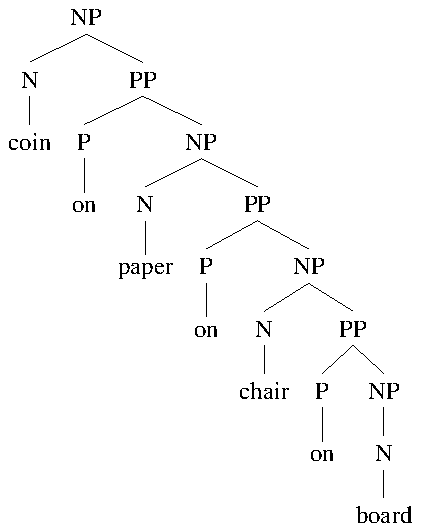
\includegraphics{figures/pullum_figure1.pdf}}
\hspace*{2em}\scalebox{0.55}{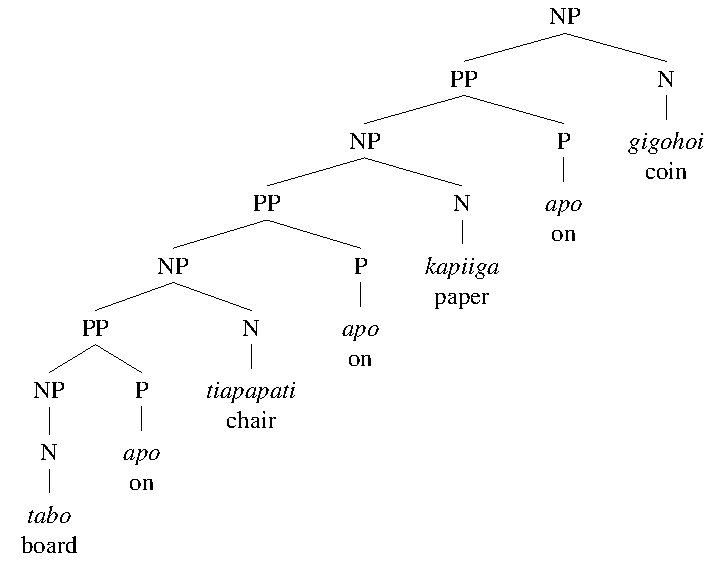
\includegraphics{figures/pullum_figure2.pdf}}

\noindent
Sandalo et al.\ have overlooked a crucial syntactic fact. Pirah{\~a} is
\textsc{not} a uniformly head-final language. As Everett noted forty
years ago, in the noun phrase `modifiers follow, while possessors normally
precede, the phrase head' (\citealt{Everett86HAL}:272). He lays out
the sequence of elements in the NP as follows (p.\,273):\footnote{\,
   See also Everett (\citeyear{Everett83}:132ff). Pirah{\~a} has no true
   numerals in the sense of names for the natural numbers, but presumably
   its vague quantity-related items like \data{b{\'a}agiso} or
   \data{{\textglotstop}a{\'\i}b{\'a}} `many',
   \data{{\textglotstop}ogi{\'\i}} `a lot', and
   \data{{\textglotstop}o{\'\i}hi} `few' take that slot in the NP.}

\medskip\noindent
(7)\quad
%%% GKP: Everett's full-size caps won't fit the page width:
%%% (POSSESSOR) + (PRO.CLITIC) + N + (MODIFIER) + (NUMERAL) + (DETERMINER)
%%% So I use small caps instead:
(\textsc{possessor}) + (\textsc{pro.clitic}) + N + (\textsc{modifier})
+ (\textsc{numeral}) + (\textsc{determiner})

\medskip\noindent
The vital point is that modifiers follow the head in NPs. So if there
were noun-modifying postpositional PPs embedded in NPs within other
such PPs, the result would be nothing like the fictive left-branching
tree in (6b). In fact there's a good reason that languages with nouns
postmodified by PPs don't allow iteration of the construction: it
yields center-embedding of the sort that poses major difficulties for
human sentence processing --- the kind seen in English center-embedded
sentences like \textsuperscript{??}\data{The children the women the
soldiers left saved protested}.

The purported phrase Sandalo et al.\ are trying to diagram would
actually come out as in (8), where I correct the transcriptions
and word identification as well as the structure.

\medskip\noindent
(8) Expected structure if Pirah{\~a} had nesting of PP modifiers in NPs

\nopagebreak[4]

\hspace*{2em}\scalebox{0.7}{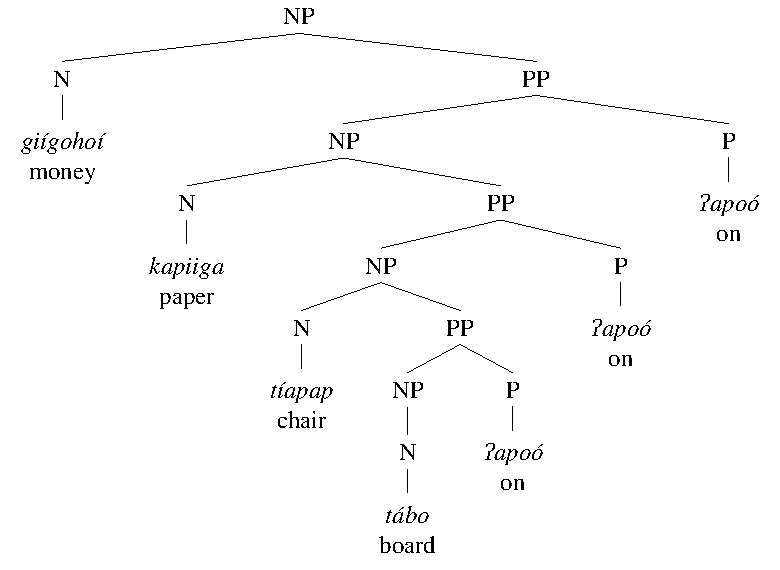
\includegraphics{figures/pullum_figure3.pdf}}

\medskip\noindent
No one has ever suggested that PPs like (8) are encountered in Pirah{\~a}
discourse, and no such structures were presented to Sandalo et al.'s
hapless informant.\footnote{\,
   Later they give a second similar structure for NPs containing PP
   modifiers which is best ignored. Their (21) on p.\,287 has nodes
   labeled `PP*' dominating other nodes with that label. On p.\,284
   they say they are using `notation adapted from traditional Kleene*
   system' [sic], but Stephen Kleene's star notation symbolizes a
   unary operation mapping a set of strings to its reflexive and
   transitive closure under concatenation. It makes absolutely no
   sense in a node label.}

It is difficult to guess what must have gone on in their experimentation
(they stress that it is to be regarded only as a pilot study). They claim
to have found that a native speaker named Iao{\'a} understood their
pronunciation of the purely fictional phrase (6b). Given that the word
they write as \textit{tiapapati} seems to be the imperative verb
\data{t{\'\i}apapa{\'a}ti}, meaning `sit down'
(\citealt{EverGibs19}:786-87), Iao{\'a} would have heard them as
saying something that meant roughly `Sit on the board. On top. On
the paper. Money.' The corrected string is given in (9):

\medskip\noindent
\begin{tabular}[t]{lccccccc}
(9)&\data{t{\'a}bo}&
    \data{{\textglotstop}apo{\'o}}&
    \data{t{\'\i}apap}&
    \data{{\textglotstop}apo{\'o}}&
    \data{kapiiga}&
    \data{{\textglotstop}apo{\'o}}&
    \data{gi{\'\i}go-ho{\'\i}} \\
   &board&on&chair&on&paper&on&money
\end{tabular}

\medskip\noindent
The most likely guess at how Iao{\'a} or any native speaker would
have parsed this would be as a list of successive PPs and a final NP,
as in (10).

\medskip\noindent
(10) Most likely native-speaker parse of (9)
\nopagebreak[4]

\quad\scalebox{0.6}{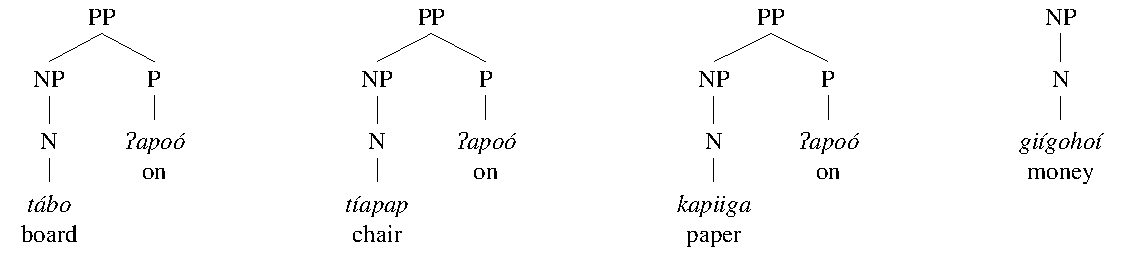
\includegraphics{figures/pullum_figure4.pdf}}

\medskip\noindent
Convinced that they had identified nested PPs in Pirah{\~a}, Sandalo
et al.\ (\citeyear{SandaloEtAl18}:289--292) proceeded to construct some
test sentences paired with pictures of alligators on mats on rocks on
beaches, and claim to have used them to produce evidence for
interpretation of nested PPs. They claim a picture of an alligator on
a mat on a beach was reliably distinguished from a picture of an
alligator on a mat beside another alligator on a beach. Further
discussion of this experiment is not really feasible; their account is
too ill-informed and confused, replete with botched transcriptions,
mistaken glosses, misidentified words (\data{tahoasi} is glossed as
`mat' when it actually means `beach' --- the word for `mat' is
\data{paah{\'o}{\'\i}s{\'\i}}), and so on.

In another experiment they tried to get Iao{\'a} to play a `game'
involving coins being put on a paper that was on a chair on a board,
or on a paper on a chair, or on a paper on a board. They note (p.\,294)
that where they supplied a string like `gigohoi kapiiga apo tiapapati
apo tabo apo' (intended to be \data{gi{\'\i}go-ho{\'\i} kapiiga
{\textglotstop}apo{\'o} t{\'\i}apap {\textglotstop}apo{\'o} t{\'a}bo
{\textglotstop}apo{\'o}}, glossed `coin paper-on chair-on board-on'),
when Iao{\'a} repeated the string `he switched the order of the PPs in
the sentence', yielding what they wrongly transcribe as `tabo apo
tiapapati apo kapiiga apo gigohoi' (`board-on chair-on paper-on coin').
This was a sign of something gone terribly wrong: Iao{\'a} was unable
to come anywhere near repeating what they thought was a single NP in
his language. But in an almost unbelievable fit of wishful thinking
(hope springs eternal in the human breast), they interpret this as
`spontaneous evidence' in favor of their hypothesis!
It seems more likely that Iao{\'a} scarcely knew what was going on,
but took their attempted PPs to be independent phrases, not
successively embedded modifiers in an NP, and repeated them back in
LIFO (last in, first out) order.

There is also a very simple semantic observation that may play a
role in interpreting the events that they take as vindication of their
hallucinated PP embedding claims. We normally take the `on' relation
between medium-sized physical objects to be transitive. Any coin on
a piece of paper on a chair is also a coin on a chair. Any alligator
on a mat on a beach is an alligator on a beach.

The most plausible conclusion from Sandalo et al.'s bungled experiments
is that Iao{\'a} parsed the fictive PPs individually, and then (with the
sharp general intelligence Everett has always noted among the Pirah{\~a})
simply guessed what the linguists wanted him to do.

\section{Sentence-length extensibility more generally}

As promised earlier, I have avoided the impenetrable thickets of confusion
found where linguists use the words `recursive' and `recursion', focusing
instead on the clearer issue of syntactic devices that can in principle
allow the construction of sentences of arbitrary length.

The issue does not have the fundamental importance that some have seen
in it. Linguistic creativity is not tied to any claim about an infinitude
of sentences, since human linguistic creativity resides mainly at the
discourse level. Nor is it tied to the ability to grasp concepts:
absence of propositional attitude verbs in a language, for example,
would not entail speakers' inability to engage in metacognition.
Everett deftly illustrates how a complex proposition with a logical
form like [\data{if} [\data{P and~Q}] ] \data{then~R} does not need
to be expressed in one sentence when he titled one of his conference
papers: `You drink. You drive. You go to jail. Where's recursion?'
\citep{Everett10}.

Everett's opponents sometimes seem to have assumed that linguistic
life with only simple main clauses would hardly be worth living.
But there is no reason to regard a language lacking unbounded sentence
extensibility devices as less useful or expressive than a language.
\citet{Kornai14} argues that the information-carrying complexity of
a finite language can actually be greater than that of an infinite one.

One way of stressing the difference between finite and infinite languages,
often touched on in undergraduate textbooks, depends on pointing out that
for a finite language the grammar could be given in the form of a simple
list of sentences. But that was never a very sensible point to harp on.
From the complexity of verbs alone (\citealt{Everett86HAL}:288--301)
it is apparent that the set of Pirah{\~a} sentences would be way too vast
even to be compiled, stored, or accessed by either a brain or a currently
imaginable computer, let alone to be of real online use either cognitively
or computationally. The grammatical complexity of Pirah{\~a} would still
pose the usual problems for the theory of language acquisition: inducing
generalizations from exposure to data would have to be involved, not just
memorizing complete utterances. As Gibson (this volume) argues, what's
important is compression of information (Kolmogorov complexity), not
infinitude.

Whether the set of all sentences in a language is finite or not is
in any case inherently difficult to settle, for a number of reasons,
and would remain so even if all of Everett's specific claims about
Pirah{\~a} syntax are accepted.

First, the lexicon has to be stipulatively fixed at some finite number
$N$ of words, though we have no clue about what $N$ might be because
new words (e.g.\ personal names) are being coined all the time, and
the interaction of agglutinative word formation and lexicalization
in languages like Turkish or Inuktitut makes it implausible that there
is any such $N$ at all.

Second, the notion `sentence' needs a clear definition; syntacticians
casually assume it is a well-understood primitive term, but it is not
easily defined at all. Separating a passage of spoken language into
sentences in a way that a different linguist would replicate is very
difficult, and beset with problems raised by false starts,
parenthetical interruptions, direct quotations, appositional
expansions, rhetorical repetitions, whatever semicolons represent in
writing, and asyndeton (coordination without coordinator words, as
in Dickens's \data{It was the best of times, it was the worst of
times, it was the age of wisdom, it was the age of
foolishness\ldots}').

Third, with regard to hypotaxis (subordination), \citet{PawlSyde00}
argue that it hardly occurs at all in spontaneous speech, even in
English, once we set aside a limited number of high-frequency partially
customizable schemata like \data{I~think~\blank}\, or \data{It depends
whether~\blank}\,, and similar formulas. This would presumably be all
the more true for languages spoken in cultures where no one writes
or reads. A few folk tales or epic poems might have a broadly fixed
(or even faithfully memorized) traditional form, but most language
use will be informal chatting, and Pawley and Syder claim that
spur-of-the-moment construction of hypotactic sentences will be rare
to nonexistent.

There are other phenomena that could introduce difficulties: NP
apposition, roughly definable as adjacent iterated NPs with the same
reference and syntactic function (\citealt{Karlsson10} cites an
attested five-NP example in Swedish); intensificatory or iconic
repetition of attributive adjectives (\data{a~big, big, big problem})
or adverbs (\data{I~really, really mean it}) or VPs \data{They hit
me and hit me and hit~me\ldots}) or NPs (\data{cows, cows, \ldots\
cows, as far as you could see}). Such possibilities are seldom noted
in reference grammars. It only study of large corpora of Pirah{\~a}
texts will tell us whether such iterable sentence-lengthening
constructions are found in the syntax of an exclusively oral language
like Pirah{\~a}.

How might we even estimate the likelihood that Pirah{\~a} truly has no
unbounded syntactic resources for sentence lengthening? A beautiful
and oddly neglected paper by \citet{WidmerEtAl17} addreses this
question. Widmer and colleagues suggest some additional methods that
could be employed to figure out the probability of a language lacking
such resources. They identify five ways in which NPs in Indo-European
languages can be lengthened by embedding other NPs inside them: stacked
genitive determiners, adjectivization-derived modifiers, modifiers
with head marking, adpositional modifiers, and simple noun
juxtaposition (I assume apposition is to be included under the latter
heading). They show that Indo-European languages have repeatedly
developed such devices and also lost them through syntactic change
over the past few thousand years.

Through a clever calculation they then assess how likely an Indo-European
language is to end up at a given time with at least one such device in
its NP syntax, concluding that it is very high indeed: they estimate
that with probability $\sim$0.98, any Indo-European language, at any
given point in its history, will have at least one grammatical device
for arbitrarily expanding NPs. As an explanatory conjecture, they suggest
that for some reason the human processing capacity finds it helpful for
there to be some such mechanism provided by the grammar.

However, they add (p.\,822): `With regard to sentence-level syntax,
it remains an open question whether syntactic recursion or simple
conjunction is preferred.' To settle it, `a larger sample of data
would be needed.' We cannot know what the answer is, or how likely
it is that any arbitrary language in the world (not just in the
Indo-European family) would have some kind of iterable
sentence-lengthening syntactic device available at all times in its
history. But suppose the probability of languages having such features
were as high as $\sim$0.99. It would still be expected, given the
7,000 languages attested in the world today, that there might be 70
languages or more in which such devices are absent. The literature
on ancient languages and languages of preliterate cultures has thrown
up quite a few candidates, as discussed in section~\ref{intro}.
Pirah{\~a} just happens to be the clearest case --- and the one that
kicked the hornets' nest politically.

\section{Conclusions}

No one should claim, in the present state of our knowledge, that we
have a good understanding of the syntax of Pirah{\~a} (or for that
matter any other language, even Standard English). The corpus study
of Pirah{\~a} syntax by \citet{FutrellEtAl16} is a sterling effort
at utilizing what materials we have (specifically, parsing texts
collected by Steven Sheldon in an effort to find evidence of
subordination), but in many ways it just underlines how woefully
unclear things are. Much more work has to be done.

That work will not be accomplished without collaborations that involve
people who (i) have no advance commitment to particular results or
empirical claims and (ii) are prepared to spend time paying close
attention to everyday usage in the Pirah{\~a} speech community. That
will mean extended residence in Pirah{\~a} villages, and consultation
with people who have substantial experience with the language.

Such people exist. Steven Neil Sheldon worked on the language from
1967 to 1976, and knows it well. Caleb Everett, Kristene Diggins,
and Shannon Russell all learned to speak and understand the language
when living in Pirah{\~a} villages as children, and their parents
Daniel Everett and Keren Madora are outsiders with unprecedented
fluency. Madora has studied the language in depth since 1977 and
still lives close to the Pirah{\~a} villages; Everett spent a total
of about eight and a half years with the Pirah{\~a} between 1977
and 2006, and made various visits thereafter, becoming fully fluent
in the language. He translated the \textit{Gospel of Mark} into it
\citep{Everett86Mark}. Yet NP\&R decided to work without having a
single conversation with any of these people.

This represents a sadly missed opportunity. If linguists like NP\&R
had applied their analytical theoretical abilities to the available
data in a collaborative spirit, drawing on the knowledge of active
speakers of the language (particularly Everett himself), new linguistic
insights might have been gained. That chance has been lost, probably
forever. They have wrecked their credibility by making it so obvious
that from the start they aimed simply to bring Everett into disrepute.
All that linguistics ended up getting out of their work was an
uninformed retrospective document review. They have divided linguists
into two irreconcilable warring camps, and made the entire discipline
of linguistics look, as it did to Tom Bartlett, like a snakepit of
hostility.

Like any scientists, linguists have a duty to maintain ethical
standards and intellectual open-mindedness --- even when someone is
claiming Chomsky was wrong about something, or when the popular
press tries to fluff up a science story into something earth-shaking
or theory-trouncing and publishes absurd overstatements.

Certainly it was ridiculous hyperbole for
\textit{New Scientist} (18 March 2006)
to call Everett's account of Pirah{\~a} `the final nail in the
coffin for Noam Chomsky's hugely influential theory of universal
grammar'. If we're honest we'll admit that Chomsky does not have
enough of a detailed theory of universal grammar to constitute a full
coffinload, and do his opponents have solid enough empirical accounts
of language acquisition to nail down the lid of such a casket anyway.

It was similarly absurd for the
\textit{Chicago Tribune} (10 June 2007)
to suggest that Everett's work is analogous to a high-school physics
teacher finding `a hole in the theory of relativity'; but we all know
that sort of thing often happens when popular news media try to cover
science. Providing better and clearer hype-free accounts of our work
to science journalists will be an enduring burden, but one that we
all have to shoulder. Calmly, and with some understanding of the
fragile and difficult business of popular journalism.

I can well imagine how irksome it has been for Chomsky to see overblown
hype about a putatively theory-shaking discovery in the jungle repeated
in scores of news sources. But that doesn't justify the petty spite of
his `charlatan' remark to \textit{Folha de S.~Paulo} in February 2009,
or his assertion that `Daniel Everett's contributions are basically
nothing' in a 2021 video interview.\footnote{\,
   \url{https://www.youtube.com/watch?v=UBla-h36ywA}}

Over the past four decades, Everett can be fairly said to have done
more for Amazonian linguistics than any other linguist now living.
His detailed descriptions of Pirah{\~a} and Wari' are lasting
contributions, as is his energetic promotion and encouragement of
descriptive work on other Brazilian languages. His basic claim about
Pirah{\~a} syntax not permitting unbounded sentence length is very
probably true. He did not deserve the years of hot-tempered public
allegations and insults (or the worse incidents of insult, hate mail,
and shouting in his face that he does not publicly report). A sector
of our field seems to have lost its moral compass over this issue.

It speaks well of Everett that never in all the years since 2005 has
he responded to his tormentors with insults or abuse: he argues points
of fact, but he refrains from accusing his enemies of scientific
misconduct, devious motives, or self-interested mendacity. For that,
and much more, we should salute him.

And as regards the validity of the accusations hurled at him by his
many opponents, none of them familiar with the lives and spoken
language of the Pirah{\~a}, I quote in conclusion the opinion of a
young Brazilian anthropologist writing recently about Pirah{\~a}
culture \citep{Felizes23}:
\begin{quote}
A rela{\c{c}}{\~a}o de Daniel e Karen Everett com os Pirah{\~a} {\'e}
algo que perdura at{\'e} aos dias atuais. Durante mais de quarenta
anos de convívio – permanente ou espor{\'a}dico – conquistaram a
reputa{\c{c}}{\~a}o de grandes amigos, de saberem bem a l{\'\i}ngua, de
serem exímios contadores de histórias e de se tornarem importantes
aliados, a quem os Pirah{\~a} geralmente recorrem para resolver
potenciais conflitos ou aprender coisas sobre o mundo dos brancos.

\noindent
[Daniel and Keren Everett's relationship with the Pirah{\~a} is something
that has endured to the present day. During more than forty years of
coexistence --- permanent or sporadic --- they gained the reputation of
being great friends, of knowing the language well, of being excellent
storytellers and of becoming important allies, to whom the Pirah{\~a}
often turn to resolve potential conflicts or learn things about the
white world.]
\end{quote}
That is the view formed by an independent third party with a personal
commitment to studying the life of the Pirah{\~a}, some who has spent time
in Pirah{\~a} villages, made the acquaintance of Keren Madora [formerly
Everett], and witnessed the consequences of the Everetts' 46 years of
friendship with the Pirah{\~a} at first hand.

\section*{Acknowledgments}
I have known Daniel Everett and his work since 1983, and gratefully
acknowledge his openness and candor during our discussions of this topic.
During the four decades we have known each other we have agreed on many
things and disagreed on many others. In writing this paper I have
confirmed claims about specific people's actions and statements from
suitable sources or personal reminiscences as far as that was possible.
I thank many friends who have spent time reading drafts, answering
my questions, helping me to verify facts, saving me from errors,
and making useful substantive suggestions. Among them are
Judith Aissen,
Ash Asudeh,
Peter Austin,
James Blevins,
Bernard Comrie,
Peter Culicover,
Lise Dobrin,
Ted Gibson,
John Goldsmith,
Randy Allen Harris,
Lloyd Humberstone,
John Joseph,
Ed Keenan,
Bob Ladd,
Pim Levelt,
Noah Ley,
Joan Maling,
John McWhorter,
Philip Miller,
Stefan M{\"u}ller,
Georgia Morgan,
David Nash,
Johanna Nichols,
Steve Piantadosi,
Steven Pinker,
Jerry Sadock,
Jeanette Sakel,
Rich Thomason,
Sally Thomason,
Tom Wasow,
Rebecca Wheeler,
Melinda Wood, and
Annie Zaenen.
Errors may remain, and they are solely mine.
Presentations of some of the content of this paper were made during
2023 at MIT, George Mason University, and the Max-Planck Institute
for Psycholinguistics in Nijmegen.
This is the version of \today.

\sloppy

\printbibliography[heading=subbibliography,notkeyword=this]

\end{document}
